\documentclass[11pt]{article} % Basic document type
\usepackage{times} % Font 
\usepackage{amsmath} % For matrices
\usepackage{amssymb}
\usepackage[section]{placeins} % Allows FloatBarrier command
\usepackage[utf8]{inputenc} % Font encoding
\usepackage[margin=1.0in]{geometry} % Adjust margins
\usepackage{graphicx} % Allows picture import
\usepackage{subcaption}
\usepackage{pdfpages} % Including pdf files 
\usepackage{setspace}
\usepackage{soul} % Highlighted text
\usepackage{fancyhdr}
\usepackage{appendix}
\usepackage{hyperref}
\usepackage{url}
\usepackage{mcode}
\graphicspath{{images/}} % Allows picture import
\pagestyle{fancy}
\fancyhf{}
\fancyhead[L]{Research \& Development of a Real-Time Object Tracking System}
\fancyhead[R]{ECSE 457}
\fancyfoot[C]{\thepage}
\renewcommand{\headrulewidth}{1pt}
\renewcommand{\footrulewidth}{1.5pt}
\newcommand{\HRule}[1][\medskipamount]{\par
  \vspace*{\dimexpr-\parskip-\baselineskip+#1}
  \noindent\rule{\linewidth}{0.2mm}\par
  \vspace*{\dimexpr-\parskip-.5\baselineskip+#1}}
\begin{document}
\begin{titlepage}
\begin{center}
\textsc{\huge McGill University}\\[1.5cm]
\textsc{\LARGE Department of Electrical \& Computer Engineering}\\[1.5cm]
\textsc{\Large ECSE 457 - Final Report}\\[3cm]
\HRule
{\huge \bfseries Research \& Development of a Real-Time Object Tracking System \\[.3cm] }
\HRule 
\vspace{1.5cm}
\noindent
\begin{minipage}{0.4\textwidth}
\begin{flushleft} \large
\emph{\Large Authors:}\\
\vspace{.2cm}
Benjamin \textsc{Brown} \\
\textit{benjamin.brown2@mail.mcgill.ca} \\
260450182 \\
\vspace{.2cm}
Taylor \textsc{Dotsikas} \\
\textit{taylor.dotsikas@mail.mcgill.ca} \\
260457719
\end{flushleft}
\begin{flushleft} \large
\emph{\Large Supervisors:}\\
\vspace{.2cm}
Warren \textsc{Gross, Prof.}\\
\vspace{.2cm}
Arash \textsc{Ardakani} 
\end{flushleft}
\begin{flushleft} \large
\emph{\Large Sponsored by:}\\
\vspace{.2cm}
\textsc{Analog Devices}\\
\end{flushleft}
\end{minipage}%
\end{center}
\end{titlepage}
\pagebreak
\section*{Abstract}
This project aimed to research object tracking algorithms, and implement the algorithm best suited to meet project requirements in both software and hardware. The software implementation used static input videos and the hardware implementation used a real-time input video stream. Phase 1 of the project focused on algorithm research and software implementation, and is documented in \cite{phase1}. Phase 2 of the project focused on hardware implementation, and this report encompasses all of Phase 2 from the design process to the final results. It was found that hardware implementation of the algorithm provides a much faster way of tracking an object when compared to the equivalent software implementation. It was also found that using a background subtraction, delta frame based algorithm to determine object position is not the best choice for real-time situations, due to the inability to cope with lighting and background variations. It was also found that while a Kalman filter does greatly improve object tracking results, it comes at a heavy cost in terms of hardware utilization.
\section*{Acknowledgments}
We would like to thank Professor Warren Gross and Arash Ardakani for overseeing this project and providing advice, insight, and direction over the course of the year. We would also like to thank Analog Devices for providing us with the Altera DE2 board needed for hardware implementation, and in particular Leah Magaldi for being our main point of contact. Finally, the example TV decoder Verilog code provided by Terasic was a major asset for hardware implementation, we would like to thank them for making it open and available to developers like ourselves. 
\pagebreak
\tableofcontents
\pagebreak
\section{Abbreviations \& Notation}
\begin{itemize}
\item[] FPGA - Field Programmable Gate Array
\item[] VGA - Video Graphics Array
\item[] HDL - Hardware Description Language
\item[] FIFO - First In First Out
\item[] SDRAM - Synchronous Dynamic Random Access Memory
\item[] SRAM - Static Random Access Memory
\item[] RAM - Random Access Memory
\item[] FSM - Finite-State Machine
\end{itemize}
\section{Introduction}
The ability to determine the position of an object in a scene is a highly relevant challenge for industries like surveillance and robotics. This task represents a challenge from an engineering perspective due to the real-time timing constraints placed on these systems, and the large amount of data that must be processed when working with video data. In order to overcome these challenges, custom hardware implementation has become an increasingly popular solution as demonstrated in \cite{1}, \cite{2}, and \cite{3}. \\\\
The goal of this project was to research and develop a real-time object tracking system, and implement this system in both software and hardware. The motive was to study computer vision fundamentals like optical flow, and learn about implementing a real-time algorithm using programmable hardware. The final system provides an accurate measurement of an object's position, meaning the system could be used in a variety of applications where this is a concern such as robotics and camera stabilization. Aside to getting the system working, other project goals included low budget, rapid prototyping, low resource utilization, and fast processing to meet real-time constraints.
\section{Background}
This section contains the prerequisite information regarding video tracking needed to understand the system architecture and design. For background information regarding the basics of video processing, Kalman filtering, fixed-point representation, and optical flow, please see \cite{phase1}.
\subsection{Moving Average Filter}
\label{sec:filter}
A moving average filter replaces the current input data sample with a mean of some number of past input data samples. The number is referred to as the moving average filter length, $N$. This type of filter is particularly useful when data samples are arriving in a time series (i.e. at constant time intervals) as it will remove outliers, creating a smoother trend in data samples. Given that $p_i$ is the current input data sample, the filtered results, $p_i'$, is given using the following equation,
\begin{equation}
p_i' = \frac{\sum_{k = i}^{i + N} p_{k-N}}{N}
\end{equation}
\subsection{Saturation Filter}
A saturation filter, in the context of this project, refers to either flooring a grayscale pixel intensity to a minimum value or ceiling the grayscale pixel intensity to a maximum value, if it is below or above a threshold. The pseudo-code for the saturation filter is given below.
\begin{lstlisting}
function [output] = saturation_filter(input, min, max, thresh)
	if (input > thresh)
		output = max;
	else
		output = min;
	end
end
\end{lstlisting} 
This makes the data set binary, in the sense that all values are one of two values, and makes data processing significantly easier. In the context of object tracking, values above the threshold indicate an object present in the scene, and values below indicate no object present.
\subsection{Determining Position}
The algorithm implemented in software, and presented in \cite{phase1}, for determining the $(x,y)$ position of an object in the delta frame used a rastor scan technique to determine the leftmost, rightmost, top, and bottom pixels. By intersecting two lines formed between these points, the center of the object can be estimated. It was found that despite the success of this algorithm in software, it would not be conducive to hardware implementation. This is mainly due to the fact that in the software implementation, data arrived in discrete frames from MATLAB's \texttt{VideoReader} class at constant time steps. In hardware implementation, data is handled at the pixel level, with a constant stream of pixels being placed in and extracted from a FIFO frame buffer storage module (to be discussed later). Thus, using an algorithm that requires an entire frame needs more memory and extra logic. A new algorithm was developed to determine the location of the object. \\\\
This algorithm assumes that pixel data arrives in binary format; either a string of all zeros representing no object present or a string of all ones representing an object present. Note that this data format is achieved by using the saturation filter just discussed. The algorithm tests if the pixel is an object pixel or not, and if it is the $x$ and $y$ coordinates of the pixel are each added to a rolling summation ($x_{sum}$ and $y_{sum}$). A counter, $n$, is also incremented. At the end of the frame, the rolling summations are divided by the counter, the position is outputted, and the three values are cleared. This algorithm is essentially just taking an average of the $(x,y)$ coordinates of the object pixels as the center of the object.
\begin{equation}
\label{eq:x}
x = \frac{x_{sum}}{n}
\end{equation} 
\begin{equation}
\label{eq:y}
y = \frac{y_{sum}}{n}
\end{equation} 
Note that this algorithm achieves best results when the object is very symmetric.
\subsection{Video Pipeline}
The phrase \textit{video pipeline} refers to a series of image processing modules that exist between the video input device (e.g. the camera) and the video output device (e.g. the display). The pipeline can be implemented in software or hardware, but for the scope of this report the pipeline will refer to hardware implementation, and modules will be referred to in the Verilog sense. Modules in the video pipeline generally consist of decoding and encoding the video data into various formats, and performing video processing (e.g. applying algorithms of interest) in the middle. Implementing a video pipeline is directly coupled with implementing an object tracking algorithm in hardware, as there are no libraries or classes to convert and store the incoming video data when working at this low of a level.
\subsection{The VGA Interface}
\label{sec:vga}
The ADV7123 High-Speed Video DAC converts three 10-bit RGB digital signals to the corresponding analog signals needed to transmit video data using the VGA interface. To give the user flexibility with timing and resolution, it does not generate the digital synchronization signals. These two signals are horizontal and vertical synchronization (sync). To properly generate these signals and thus drive the VGA interface, the VGA timing specifications must be understood. \\\\ 
A VGA display generates images using a rastor scan technique. The display is a grid of pixels, and each pixel is displayed individually starting at the top left corner, moving left to right in rows, and ending in the bottom right corner. This operation occurs at a speed known as the refresh rate. The refresh rate is fast enough such that the user perceives an entire image display instantaneously, despite the fact that the image is being displayed discretely per pixel. Due to the motion just described, VGA timing specifications are described in terms of horizontal (i.e. the rows) and vertical (i.e. the number of rows) parameters. VGA resolution is described in terms of the number of visible pixels in a single row, and the total number of visible rows in the display. It is important to note that the number of visible pixels and rows is less than the total number of pixels and rows, as there are blanking periods due to timing constraints. The final term that should be defined is the pixel clock, $f_{pixel}$. The pixel clock is used to count each pixel in the grid, and is much faster than the refresh rate. In fact, the refresh rate of a VGA display can be related to the pixel clock and VGA resolution,
\begin{equation}
f_{refresh} = \frac{f_{pixel}}{H_{pixels} \times V_{lines}}
\end{equation}
 Figure \ref{fig:vgaTiming} shows the timing specifications, and has four notable regions: front porch, back porch, sync, and active video \cite{vga}. 
\begin{figure}[h]
\centering
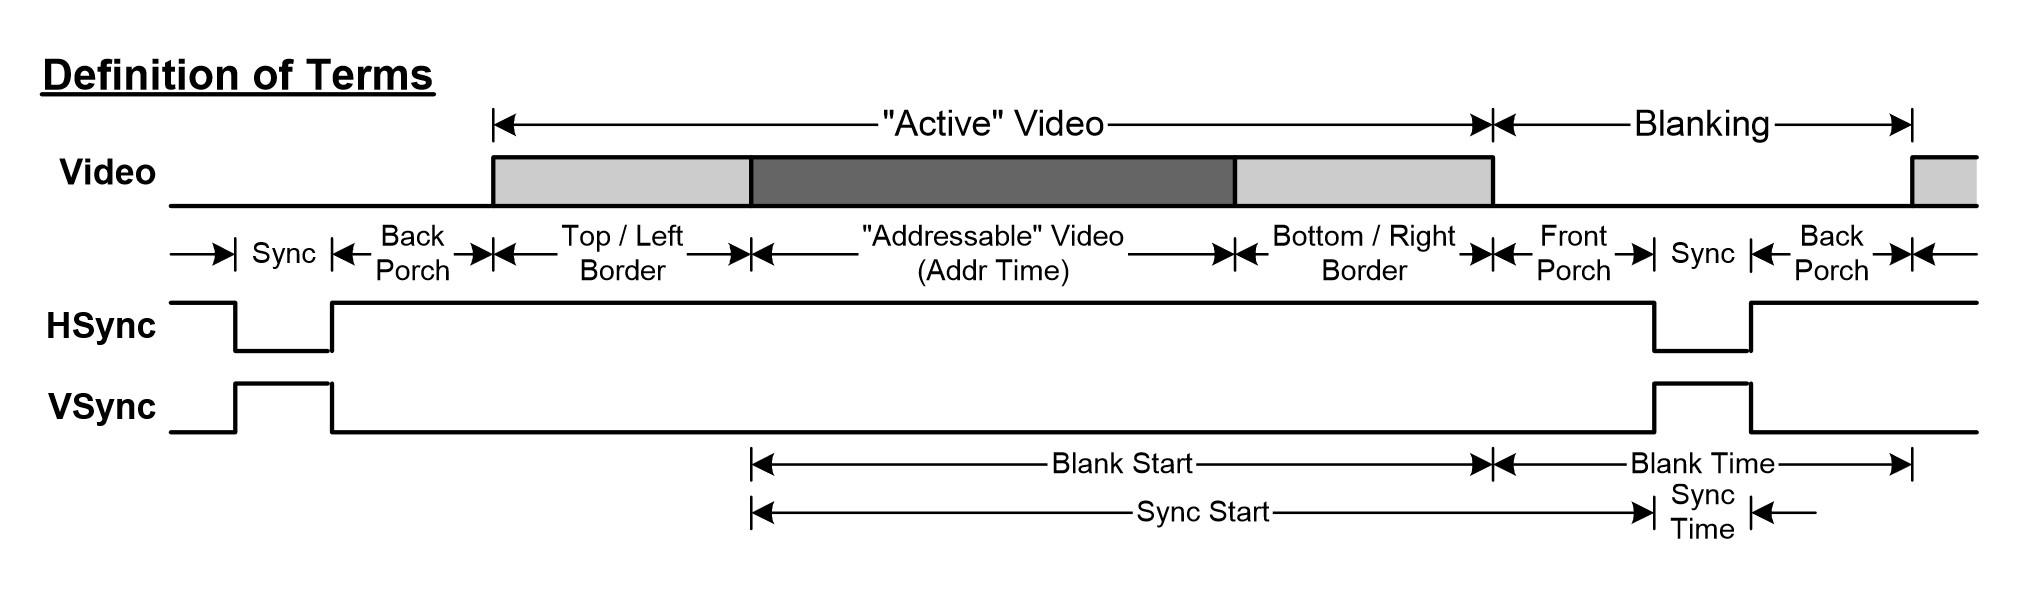
\includegraphics[width=0.8\textwidth]{./images/vgaTiming.jpg}
\caption{VGA Timing Signals \cite{vga}}
\label{fig:vgaTiming}
\end{figure}
As the figure shows, the front porch, back porch, and sync regions form what is known as the blanking period, since no valid video data is displayed during this period. The horizontal sync signal must be pulsed (high or low depending on polarity) prior to the valid data is displayed on each row, for a specific amount of time depending on resolution. Similarly, the vertical sync signal must be pulsed prior to the entire frame is displayed. For the typical $640 \times 480$ VGA resolution, the timing constraints are shown in Table \ref{table:vga}. \\\\
\FloatBarrier
\begin{table}[h]
\centering
\caption{$640 \times 480$ VGA Timing Specifications \cite{vga}}
\label{table:vga}
 \begin{tabular}{ | p{4cm} | p{4cm} | p{4cm} |} \hline
 \textbf{Region} & \textbf{Time} & \textbf{Pixels} \\ \hline
Hor. Front Porch & .636 us & 16 \\ \hline
Hor. Sync Period & 3.813 us & 96\\ \hline
Hor. Back Porch & 1.906 us & 48\\ \hline
Hor. Visible & 25.422 us & 640\\ \hline
Ver. Front Porch & 0.317 ms & 10 \\ \hline
Ver. Sync Period & 0.064 ms & 2 \\ \hline
Ver. Back Porch & 1.048 ms & 33 \\ \hline
Ver. Visible & 15.523 ms & 480\\ \hline
\end{tabular}
\end{table}
\FloatBarrier
\textit{Note: Some specifications, such as \cite{vga}, add two more regions denoted left and right borders. However, since they are functionally irrelevant for this application, they have been lumped into the front and back porches respectively.}
\section{Requirements}
Due to the fact that the scope of the project did not change between Phases 1 and 2, the requirements listed in this section are largely based off of the Phase 1 report \cite{phase1}. Some additional requirements were added at the beginning of Phase 2 when hardware implementation became clearer.
\subsection{Time Frame}
The project shall be completed by December 2015. The project will be broken into two phases. Phase 1 of the project will be January - April 2015, and Phase 2 of the project will be September - December 2015.
\subsection{Algorithm}
An algorithm shall be chosen such that the system is capable of tracking an object that is in motion, in real-time. The algorithm will be simple enough such that it can be implemented in hardware within the project's duration and within the scope of the author's skills. To ensure this, the chosen algorithm will contain basic operations in order to ease hardware implementation. The algorithm will be chosen during Phase 1 of the project.
\subsection{Software}
Software implementation of the algorithm shall be performed during Phase 1 of the project to act as a proof of concept for the algorithm, and to understand the strengths and weaknesses of the algorithm. Software implementation shall be performed in MATLAB. Upon completion, the software will be able to track an object in motion with a clear and visible cursor, for an input video that satisfies all assumptions and prerequisite conditions the algorithm may have. 
\subsubsection{Floating-Point}
The first iteration of the software implementation shall be in floating-point to provide a high-level structure of the algorithm. The software shall not have any dependencies on MATLAB (i.e. use built in functions) with the exception of simple helper functions such as \texttt{eye}, \texttt{zeros}, \texttt{round}, and \texttt{fix}. MATLAB's \texttt{VideoReader} and \texttt{VideoWriter} class may be used for I/O.
\subsubsection{Fixed-Point}
The second iteration of the software implementation shall be in fixed-point to make hardware implementation easier and more efficient. No values in the fixed-point software shall have fractional portions (e.g. reals, floats, or doubles) with the exception of constants declared directly before conversion and preparing data for MATLAB's \texttt{VideoWriter} class as output.
\subsection{Hardware}
Hardware implementation of the algorithm shall be performed during Phase 2 of the project. The completed hardware implementation of the algorithm shall be the final system. The system will contain embedded hardware which the algorithm has been implemented on. The system will include a video camera providing a live feed of the chosen scene. Upon completion, the system will be able to track an object in motion in real-time and identify the object in motion on a display with a clear and visible cursor. All components of the system shall be as low priced as possible.
\subsubsection{Platform}
The system hardware shall be an Altera DE2 breakout board. This breakout board contains video input/output peripherals, off-chip memory, and an FPGA (Altera Cyclone IV) that contains more than enough resources for the system.
\subsubsection{Method}
The system hardware shall be implemented using Verilog HDL. The sample designs included with the Altera DE2 breakout board include Verilog modules for video input decoding. In order to utilize these resources and avoid mixing languages, Verilog is the logical choice.
\section{Design}
\label{sec:design}
The hardware implementation design process was organized into experiments. Each experiment focused on investigating, implementing, or integrating a specific function into the overall system. The experiments were chronological, and built on work from the previous experiments. This section has been organized in the same chronological fashion, in order to explain and justify the system design in the manner it was developed.
\subsection{Generating VGA Output}
The first experiment was focused on generating an arbitrary VGA output using the Cyclone IV FPGA and the ADV7123. Section \ref{sec:vga} explained the motive and theory behind this. The module \texttt{vga\_sync.v} was written to implement the VGA functionality. The module takes as input the 27 MHz global clock, the global asynchronous reset, and the RGB data. The module drives the following bus of signals as an output:
\begin{itemize}
\item \texttt{VGA\_HS} - Horizontal sync pulse, driven directly to the VGA interface.
\item \texttt{VGA\_VS} - Vertical sync pulse, driven directly to the VGA interface.
\item \texttt{VGA\_R, VGA\_G, VGA\_B} - 10-bit RGB data, driven to the ADV7123.
\item \texttt{VGA\_BLANK\_N} - ADV7123 control signal, driven to the ADV7123.
\item \texttt{VGA\_SYNC\_N} - ADV7123 control signal, driven to the ADV7123. 
\item \texttt{VGA\_CLK} - ADV7123 pixel clock, driven to the ADV7123.
\end{itemize}
To achieve the necessary timing specifications for the $640 \times 480$ resolution discussed in section \ref{sec:vga}, two counters are implemented in hardware: one to count the pixels in a row, and another that counts the number of rows. The counters are used to drive the \texttt{VGA\_HS} and \texttt{VGA\_VS} signals for the specific synchronization periods. These counters also act as the primary way to track the position of the current pixel in the system, so the signals are sent to module outputs as well. The RGB color values are simply piped through the module to the ADV7123 when the counters are in the visible portion of the VGA timing. The design of this module was heavily based on the example \texttt{VGA\_Ctrl.v} module provided by Terasic with the DE2 board. \\\\
Module verification was done qualitatively, and the top-level module for this experiment simply mapped some specific color values to the buttons on the DE2 board. By connecting the DE2 board to a VGA display, we could verify the module's functionality by observing if the expected colors showed when the buttons were pressed.
\subsection{Simple Video Pipeline}
\label{sec:pipe}
The next logical step after getting video output working was to get video input working as well. Fortunately, Terasic provides an example Verilog design for a video input/output system on the DE2 board. Entitled the \textit{TV Decoder} example, it uses ADV7123 and the ADV7181, a multi-format video decoder integrated circuit (which also resides on the DE2 board), to display a live, color video feed on a VGA display. Due to the lack of parameters, organization, and comments in the example code, it was not simple to decipher the function of each module in the example pipeline. However, we were able to strip down the video pipeline and organize it an understandable way. This process consisted of removing various modules and logic, and observing the effect on the overall system performance (i.e. the quality of the video stream). Figure \ref{fig:basicPipe} shows the minimal pipeline needed to achieve a stable, live video feed.\\\\
\FloatBarrier
\begin{figure}[h]
\centering
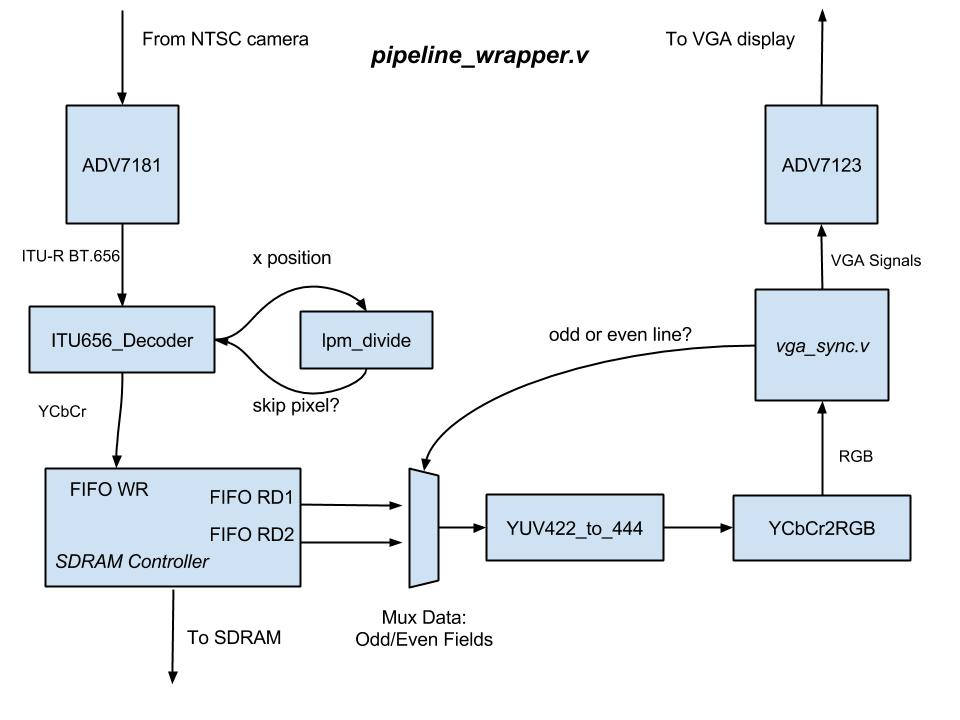
\includegraphics[width=0.5\textwidth]{./images/demoPipeline.jpg}
\caption{Basic Video Input/Output Pipeline}
\label{fig:basicPipe}
\end{figure}
\FloatBarrier
The input video stream of the camera used is NTSC format. The analog NTSC signal enters the ADV7181 via an RCA (yellow) connector on the DE2 board, and gets converted into an 8-bit, serial stream of digital data which is encoded using the ITU-R BT.656-5 protocol. This protocol encodes pixel values in interlaced (only even or odd rows) YCbCr format, using horizontal and vertical synchronization signals for timing references \cite{itu}. The low-level details of how the serial data gets converted to YCbCr pixel color values are not important, as the Terasic \texttt{ITU656\_Decoder.v} module abstracts this away and deals with the protocol. The division module is used to downsample the input video from $720 \times 480$ to $640 \times 480$ to match the VGA display. After this, the YCbCr pixel data is stored in the SDRAM frame buffer. The SDRAM frame buffer is a set of Verilog modules written by Terasic that abstract the off-chip SDRAM as a FIFO buffer. The FIFO has one write side, where data enters after the \texttt{ITU656\_Decoder.v} module, and two read sides, which are used to extract the data in a non-interlaced format. The multiplexer at the output of the frame buffer in Figure \ref{fig:basicPipe} illustrates this logic. The first half of the addressable space in the frame buffer stores the odd lines, and the second half stores the even lines. The data is extracted from one of these address spaces depending on the last bit of the VGA display row counter (i.e. the current VGA vertical position). The pixel data is upsampled and converted to RGB, and finally displayed using the VGA module discussed in the previous section. This video pipeline was wrapped in module called \texttt{pipeline\_wrapper.v} for future use, and also was commented and parameterized for readability.
\subsection{Modified Video Pipeline \#1}
\label{sec:modPipe}
Modifications would need to made to the video pipeline just presented in order to make it compatible with our algorithm. The first step in the object tracking algorithm is to convert the RGB pixel colors to grayscale, and working with the YCbCr color space is not desirable. Also, decoupling the input video decoding from the frame buffer would give more design flexibility. Based on these factors, it was determined that a video pipeline that resembles Figure \ref{fig:algoPipe} would be more ideal for integrating the object tracking algorithm. To implement this video pipeline, the upsampling and RGB conversion was pushed further upstream, before the SDRAM frame buffer. Then the Terasic modules \texttt{ITU656\_Decoder.v}, \texttt{YUV422\_to\_444.v}, and \texttt{YCbCr2RGB.v} were wrapped into a module called \texttt{Video\_Input.v}. This decoupled all video decoding from the rest of the pipeline. \\\\
\FloatBarrier
\begin{figure}[h]
\centering
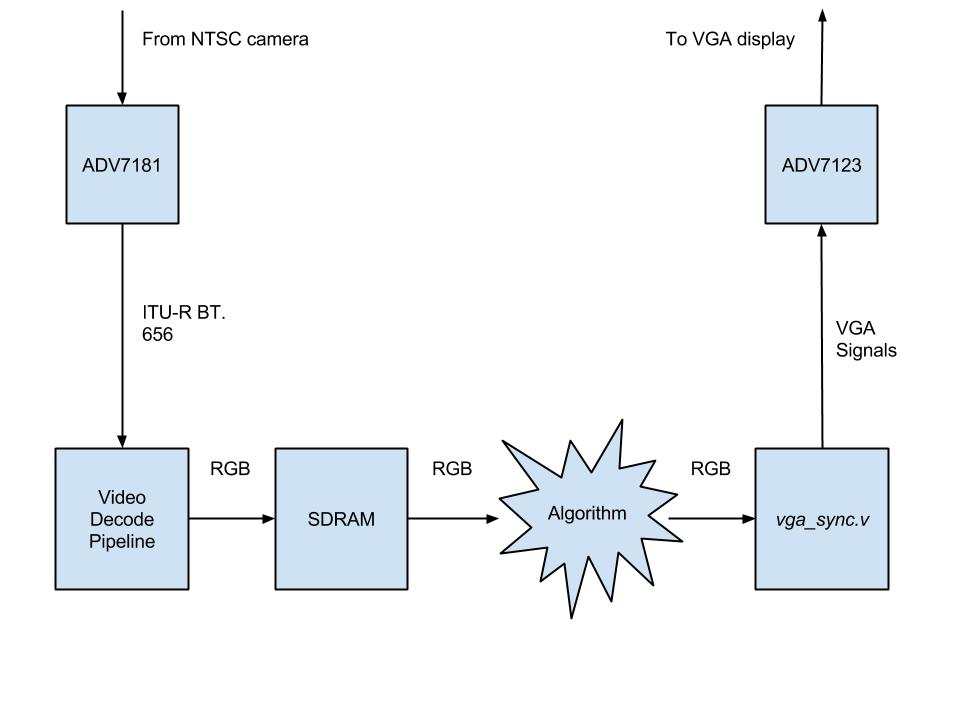
\includegraphics[width=0.6\textwidth]{./images/desired_pipeline.jpg}
\caption{Video Pipeline - Algorithm Integration}
\label{fig:algoPipe}
\end{figure}
The only major issue with this pipeline modification is the amount of data that must be manipulated when using RGB. The YCbCr pixel data that was initially being stored required 16-bits, which conveniently is the width of the SDRAM data bus. After conversion to RGB, there are three 10-bit values that must be stored in the frame buffer. Initially this dealt with by truncating the 30-bit RGB representation to high-color representation, which uses 16-bit RGB with an extra bit for green. Eventually, the grayscale conversion (to be discussed) was moved upstream before the SDRAM frame buffer, since the 30-bit RGB representation gets converted to 10-bit grayscale anyways. This modification impacted performance, in the sense that the output video was now either almost or entirely grayscale looking, but it saved logic and memory.
\subsection{RGB to Grayscale Conversion}
The purpose of this module is to convert RGB values into a single grayscale value. The sample video pipeline provided by Terasic (encapsulated into the "Video Input" module) outputs red, green, and blue pixel data into separate 10-bit registers. For simplicity in thresholding, filtering, and subsequent delta frame generation, it was not necessary to handle 3 channels of data. Converting to a single grayscale value would be sufficient for the rest of the algorithm's implementation. A grayscale value, or luminance $Y$, is achieved by performing a weighted sum of the RGB values,
\begin{equation}
Y =  0.2126\times R + 0.7152\times G + 0.0722\times B
\end{equation}
The coefficients represent the measured intensity perception of typical human eyesight. The resulting grayscale value will be in the range from 0 (total black) to 1023 (total white). This equation had to be adjusted for fixed point arithmetic since it uses fractional coefficients. A fractional width of 6 was used. The coefficients were converted to binary and left shifted by 6. The output grayscale value only maintains the most significant 10-bits of the calculation, essentially slicing the fractional portion to obtain the correct result. The equation is performed when a valid data signal is enabled by the previous "Video Input" module. A valid out signal was also introduced to maintain synchronization for the next module in the pipeline. This signal is enabled when valid input data is ready. 
\subsection{Storing the Base Frame}
As demonstrated in \cite{phase1}, the object tracking algorithm is entirely dependent on generating the delta frame, which is the grayscale difference between the the current frame and the base frame (i.e. the scene background). A method for acquiring the current frame was demonstrated in section \ref{sec:pipe}, using the SDRAM FIFO frame buffer. To acquire the base frame in a method conducive to the algorithm, the following requirements needed to be met:
\begin{itemize}
\item The base frame must be stored (i.e. latched) at a time determined by the user. It must be able to be latched multiple times.
\item The base frame must persist in memory while the system is powered on.
\item The base frame storage must have capacity for $640*480$ pixels with 2 bytes of data per pixel. This is 614,400 bytes of memory.
\end{itemize}
Since the SDRAM is already in use, another form of memory needed to be employed. Available resources on the DE2 board are SRAM and flash memory, as well as distributed RAM on the FPGA itself. Attempting to route that much RAM on the FPGA seemed like it could cause timing issues, and since the SRAM interface appeared to simpler than flash, a design decision was made to use the SRAM to store the base frame. The SRAM has 1 megabyte of storage with a 16-bit data bus \cite{sram}, which is a benefit since it matches the data width of the SDRAM. \\\\
The SRAM has a large bus of signals that must be driven by the FPGA. In order to simplify this process, a SRAM controller module was written to wrap the SRAM bus as a simple RAM interface. The simplest implementation of a block RAM needs only a few signals:
\begin{itemize}
\item Write Enable - Input: \texttt{wen}
\item Address - Input: \texttt{addr}
\item Input Data - Input: \texttt{din}
\item Output Data - Output: \texttt{dout}
\end{itemize}
Sometimes an overall enable signal is used, but this was not necessary. These signals, as well as a clock and reset, define the input/output signals for the SRAM controller that was implemented in the module \texttt{sram\_wrapper.v}. This module is quite simple, and simply drives the signals according to the datasheet specifications in \cite{sram}. The only challenge in developing this module was figuring out how to using the bidirectional data port, \texttt{SRAM\_DQ}, which required using two internal registers and three flip-flops. \\\\
The write operation, and general control flow, was verified through simulation. A testbench was written to drop multiple data and address values in series into the wrapper to observe it's operation. Unfortunately, the read operation could not be verified through simulation since we did not have a HDL model of the SRAM available to us. Verification of the read operation had to be put off until system integration.
\subsection{Modified Video Pipeline \#2}
The next step in the design process was incorporating the previous two modules, RGB to grayscale conversion and the SRAM controller, into the video pipeline. Upon successful integration, it would be possible to view the delta frame (i.e. the object pixels) on the display. \\\\
The first step was integrating the SRAM controller into the video pipeline. After some experimentation, it was determined that the SRAM should be placed after the SDRAM frame buffer in order to decouple it from the video decoding process. The SRAM address is determined by a concatenation of the x and y addresses of the VGA display. The write enable is mapped to a user controlled switch. The RAM interface portion of the SRAM wrapper module instantiation is shown here:
\begin{verbatim}
	// Wrapper Signals
	.wen  (~KEY[1]),
	.addr ({vga_x[9:0], vga_y[9:0]}),
	.din  (sdram_output),
	.dout (sram_output),
\end{verbatim}
Initially it was suspected that there would need to be constraints on how long the write enable signal was applied, in order to ensure that a full frame had been stored into the SRAM. However this was found to be unnecessary, as the user will almost certainly hold the write enable button for more than a 16 ms period (60 Hz frame rate), and assuming the base frame remains constant while the button is held, any overwriting of the previous base frame would not matter. \\\\
The initial plan for integration of the RGB to grayscale conversion module was to place one instance after both the SDRAM and SRAM outputs. This would constantly convert the current and base frames to grayscale for delta frame computation, and would allow the system to still display color output (the grayscale would just be for computation, and the SDRAM color output would still be sent to the VGA display). However, since the 30-bit RGB had already been truncated to 16-bit high color for data width constraints (as discussed in section \ref{sec:modPipe}), the result still looked somewhat grayscale anyways. So it was decided to push the module before the SDRAM frame buffer, and just work with 10-bit grayscale for both computation and display. This decision also means that only one instance of the module is required instead of two, which saves FPGA resources. Figure \ref{fig:pipe2} shows the new video pipeline after these two modules were integrated, and a module to compute the delta frame which will be discussed next.
\begin{figure}[h]
\centering
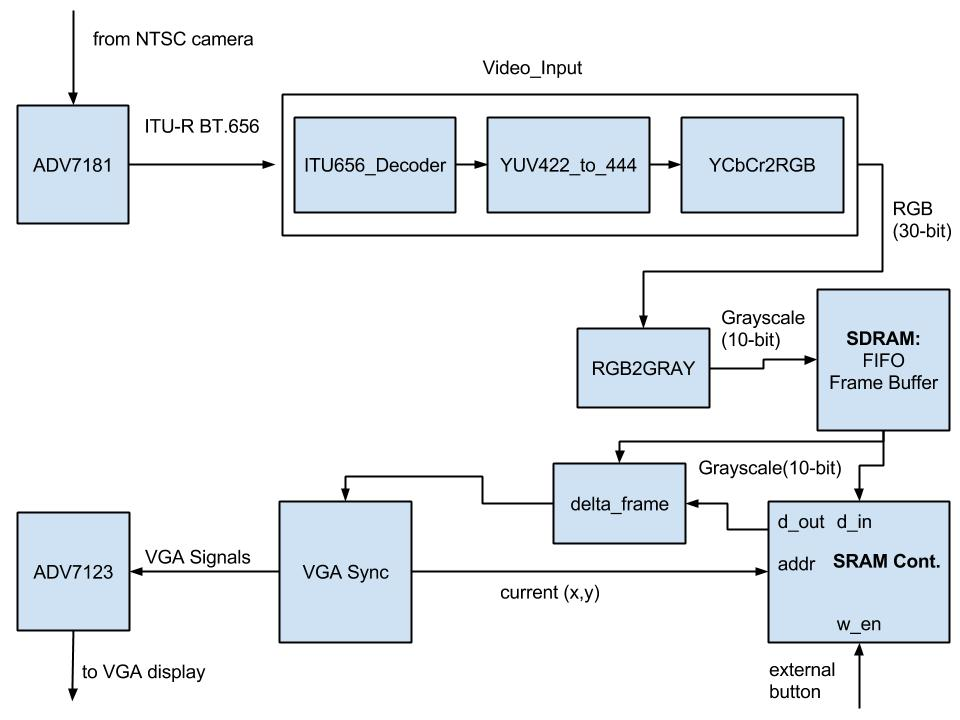
\includegraphics[width=0.6\textwidth]{./images/new_pipeline_2.jpg}
\caption{Video Pipeline - Delta Frame System}
\label{fig:pipe2}
\end{figure}
\subsubsection{Delta Frame Generation}
The module \texttt{delta\_frame.v} constantly computes the difference between the current frame (from the SDRAM frame buffer) and the base frame (from the SRAM). An example of the result the delta frame produces is shown in Figure \ref{fig:delta}.
\begin{figure}
\centering
\begin{subfigure}{.5\textwidth}
  \centering
  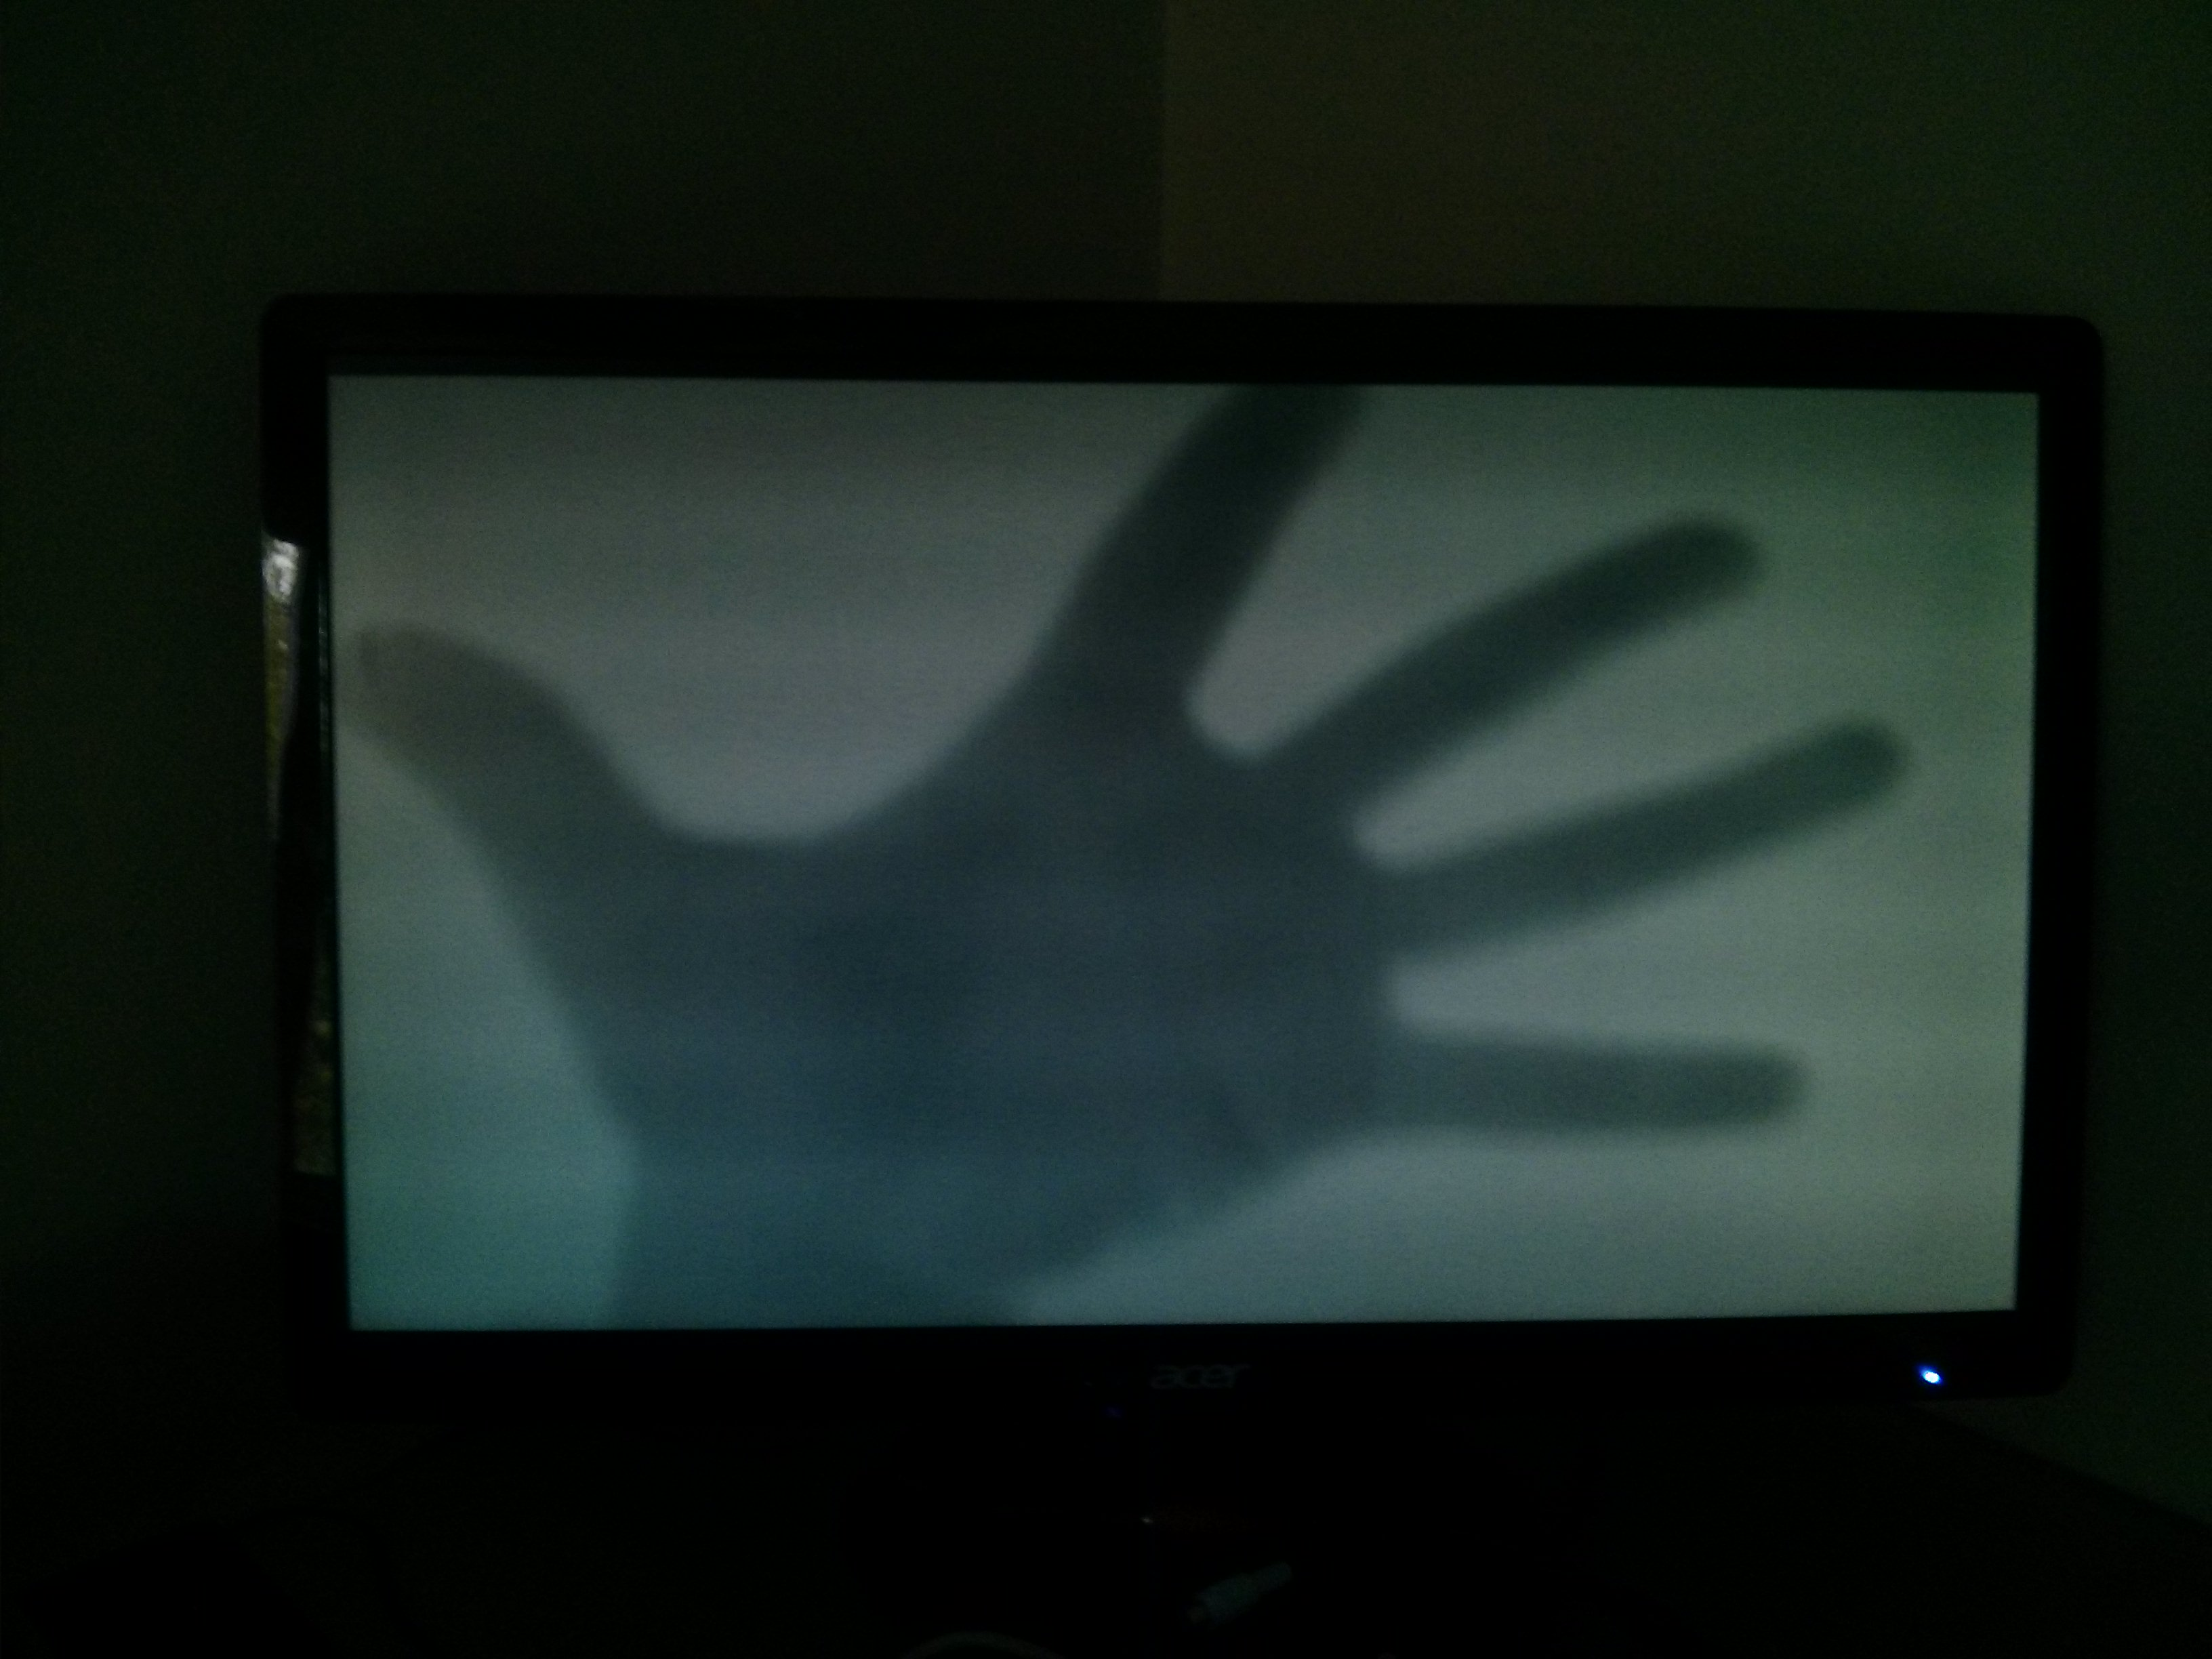
\includegraphics[width=.6\linewidth]{./images/delta_frame_1}
  \caption{Object (hand) in the base frame}
\end{subfigure}%
\begin{subfigure}{.5\textwidth}
  \centering
  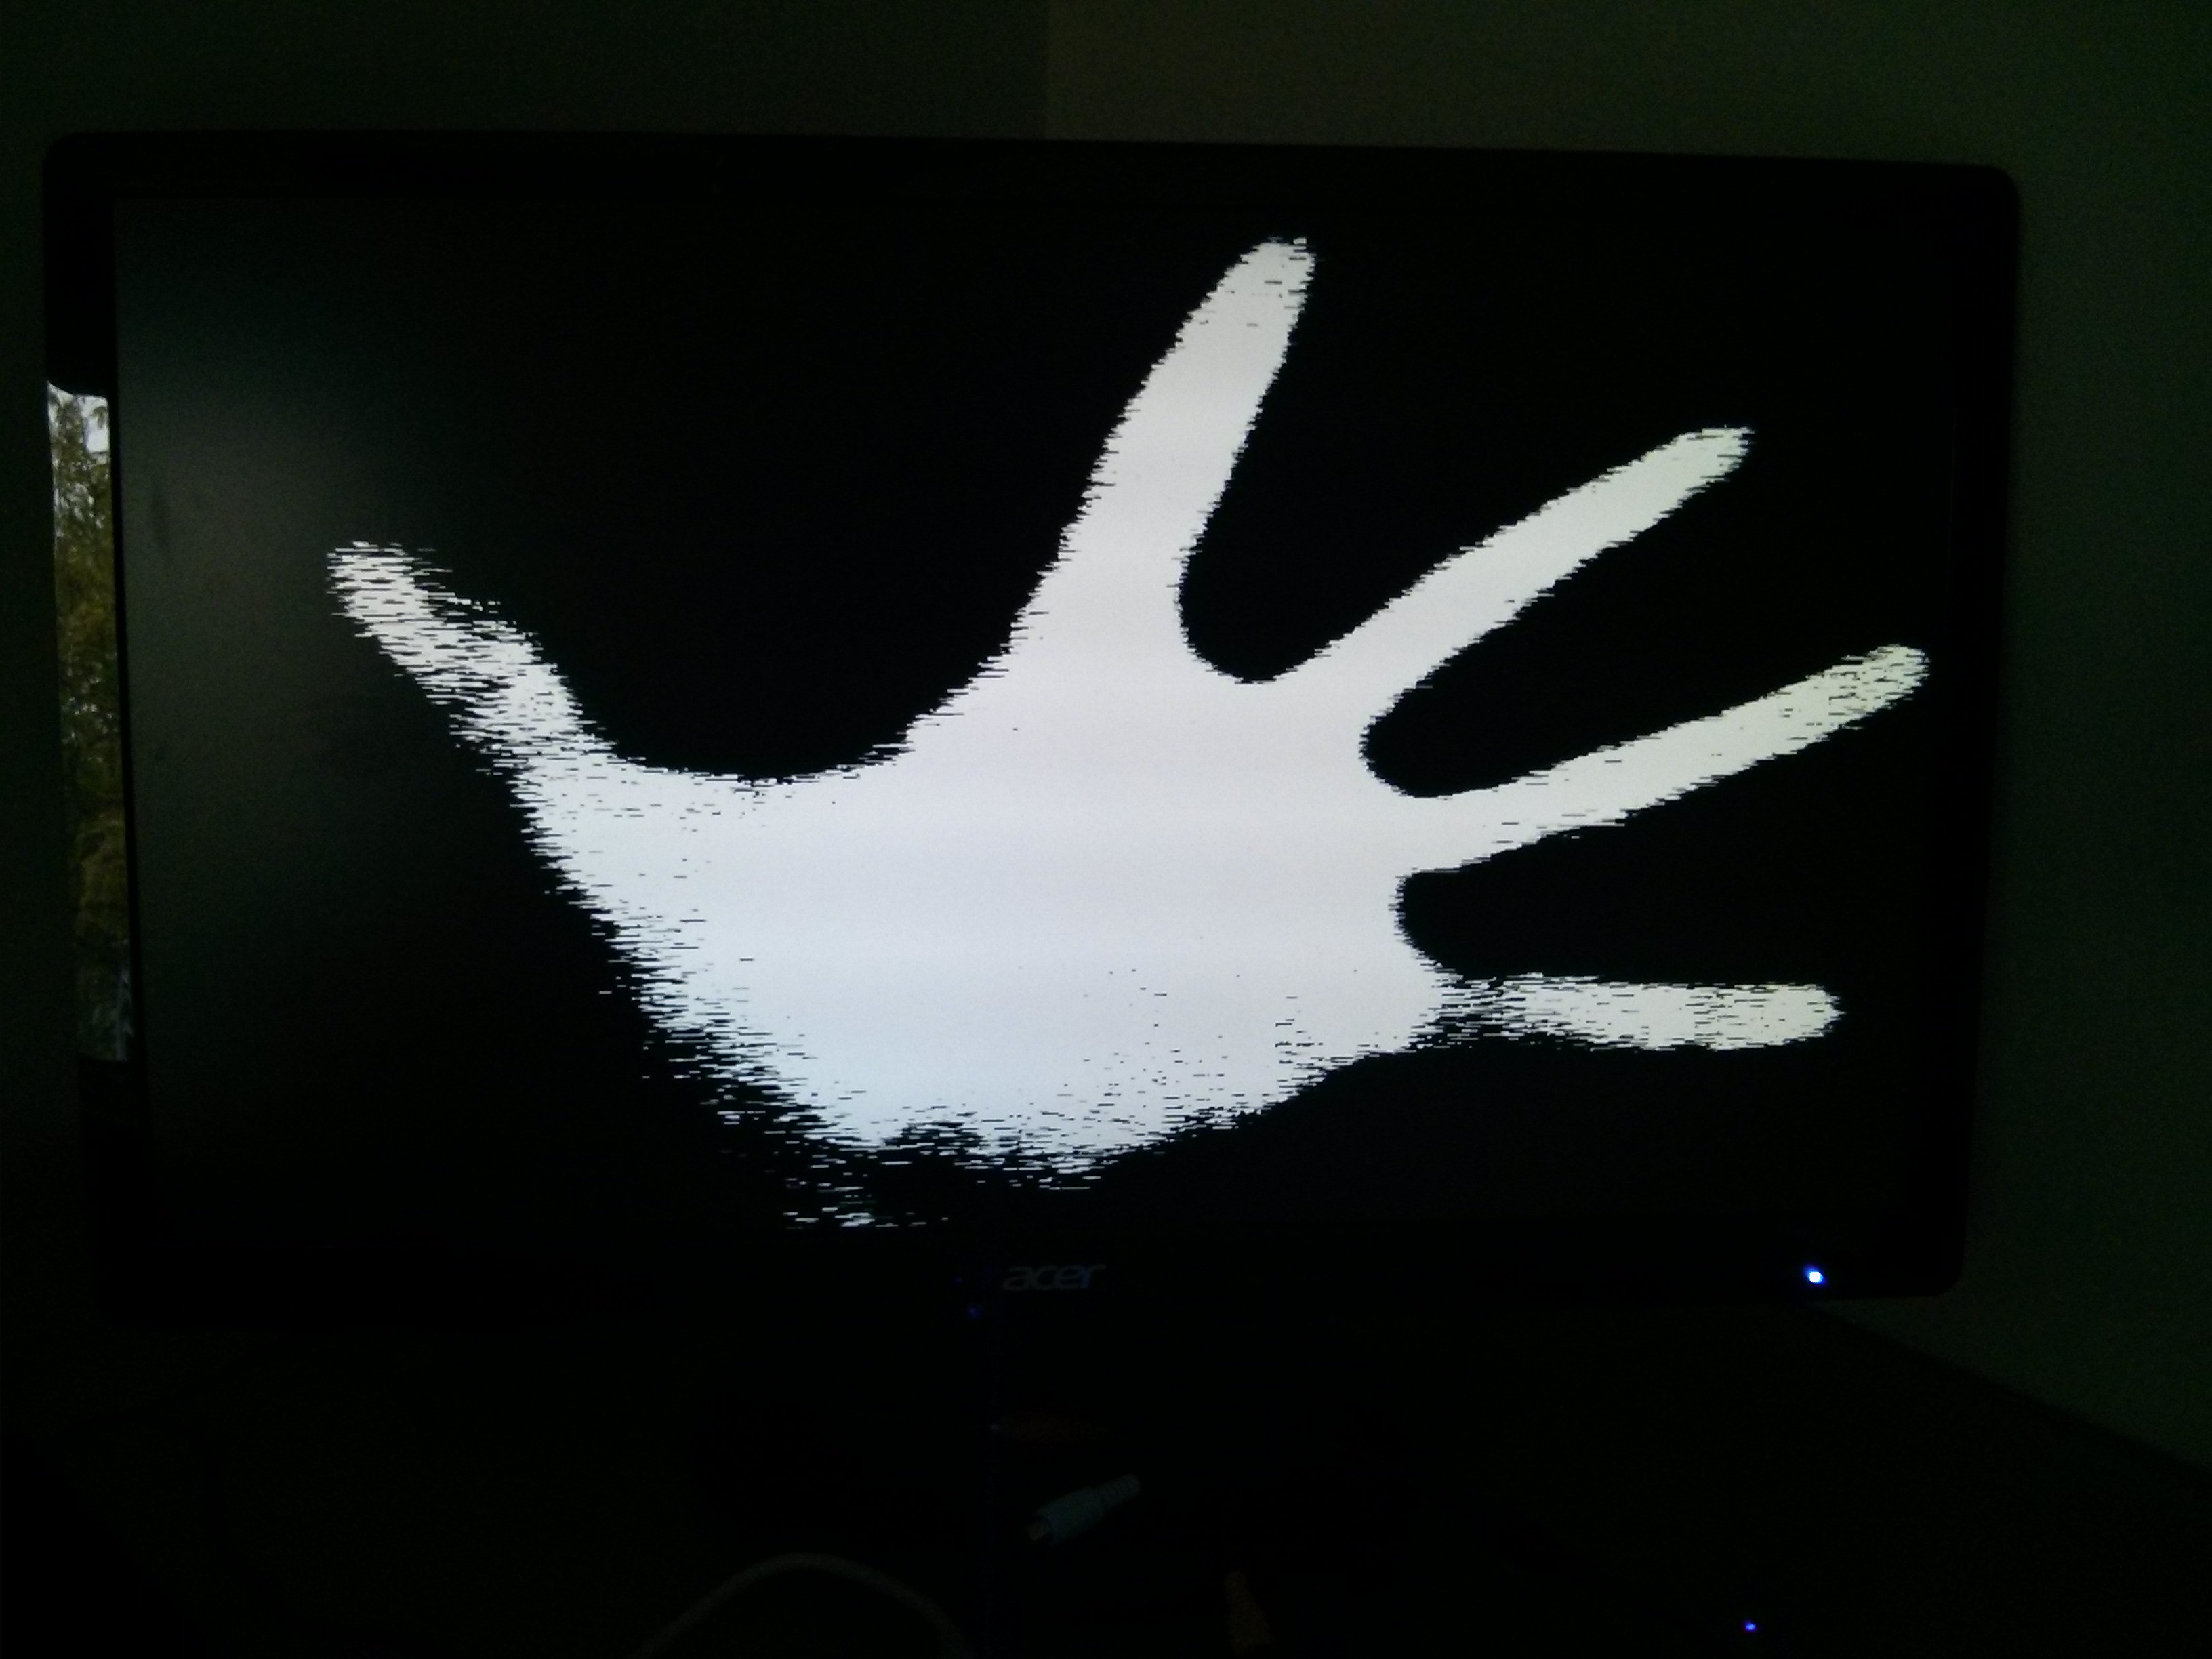
\includegraphics[width=.6\linewidth]{./images/delta_frame_2}
  \caption{Delta frame representation of the object}
\end{subfigure}
\caption{Delta Frame Example}
\label{fig:delta}
\end{figure}
This module is very straight forward, but does have a few features that are worth noting. First, the delta frame is taken to be an absolute value difference, since negative pixel intensity would not make sense. A simple implementation of an absolute value in Verilog is done with the following code:
\begin{verbatim}
if (curr_frame > base_frame)  int_delta_frame <= curr_frame - base_frame;
else                          int_delta_frame <= base_frame - curr_frame;
\end{verbatim}
The delta frame looks considerably better, and more importantly data processing is significantly easier if all the pixels in the delta frame are binary. Meaning each pixel in the delta frame is either 0 (black), representing no object present or 1023 (white), representing an object present. To accomplish this, a saturation filter was implemented in the delta frame. This means that if the difference between the two frames is above a predetermined threshold, the value is set to a string of all ones, and otherwise it is set to a string of all zeros. The Verilog code to implement this is shown here, with the parameter \texttt{COLOR\_WIDTH} representing the number of bits in the binary string:
\begin{verbatim}
assign delta_frame = (delte_frame > threshold) ? 
						{COLOR_WIDTH{1'b1}} :
						{COLOR_WIDTH{1'b0}};
\end{verbatim}
\subsubsection{Moving Average Filter}
Since the object position is entirely dependent on the delta frame, making sure the delta frame does not contain small variations in light and background is very important to the system. In software implementation during Phase 1, mean and median filters were applied to the delta frame to remove spurious object values. Since the data flow is by pixels and not by individual frames, these filters cannot be easily implemented in the video pipeline. A moving average filter, explained in section \ref{sec:filter}, is a much better choice for this system, since it will only require storing the as many past pixels as the filter length, and it doesn't require any \textit{a priori} knowledge about the frame. A moving average filter was implemented in the module \texttt{delta\_frame.v}. Using an array and the \texttt{generate} keyword in Verilog allows for a very tight and simple implementation of this filter:
\begin{verbatim}
generate 
for (c = 0; c < FILTER_LENGTH; c = c + 1) begin: moving_avg_filter
    always @(posedge clk or negedge aresetn) begin
        if (~aresetn)           old[c] <= 'd0;
        else if (~is_not_blank) old[c] <= 'd0;
        else if (counter == c)  old[c] <= int_delta_frame;
        else                    old[c] <= old[c];
    end
end
endgenerate

always @* begin
    sum = 'd0;
    for (i = 0; i < FILTER_LENGTH; i = i + 1)
        sum = sum + old[i];
end

assign avg = sum / FILTER_LENGTH;
\end{verbatim}
The \texttt{counter} variable constantly counts from 0 to the filter length. Integer division can be applied to the sum since precision is not of a concern. The result is put into the saturation filter instead of the raw difference, to provide a smoother result. Figure \ref{fig:filter} shows the delta frame representation of a plain wall base frame before and after the moving average filter. Since there is no object in the frame, an entirely black screen is the ideal result. It was experimentally determined that a filter length of 20 gave the best results.
\begin{figure}
\centering
\begin{subfigure}{.5\textwidth}
  \centering
  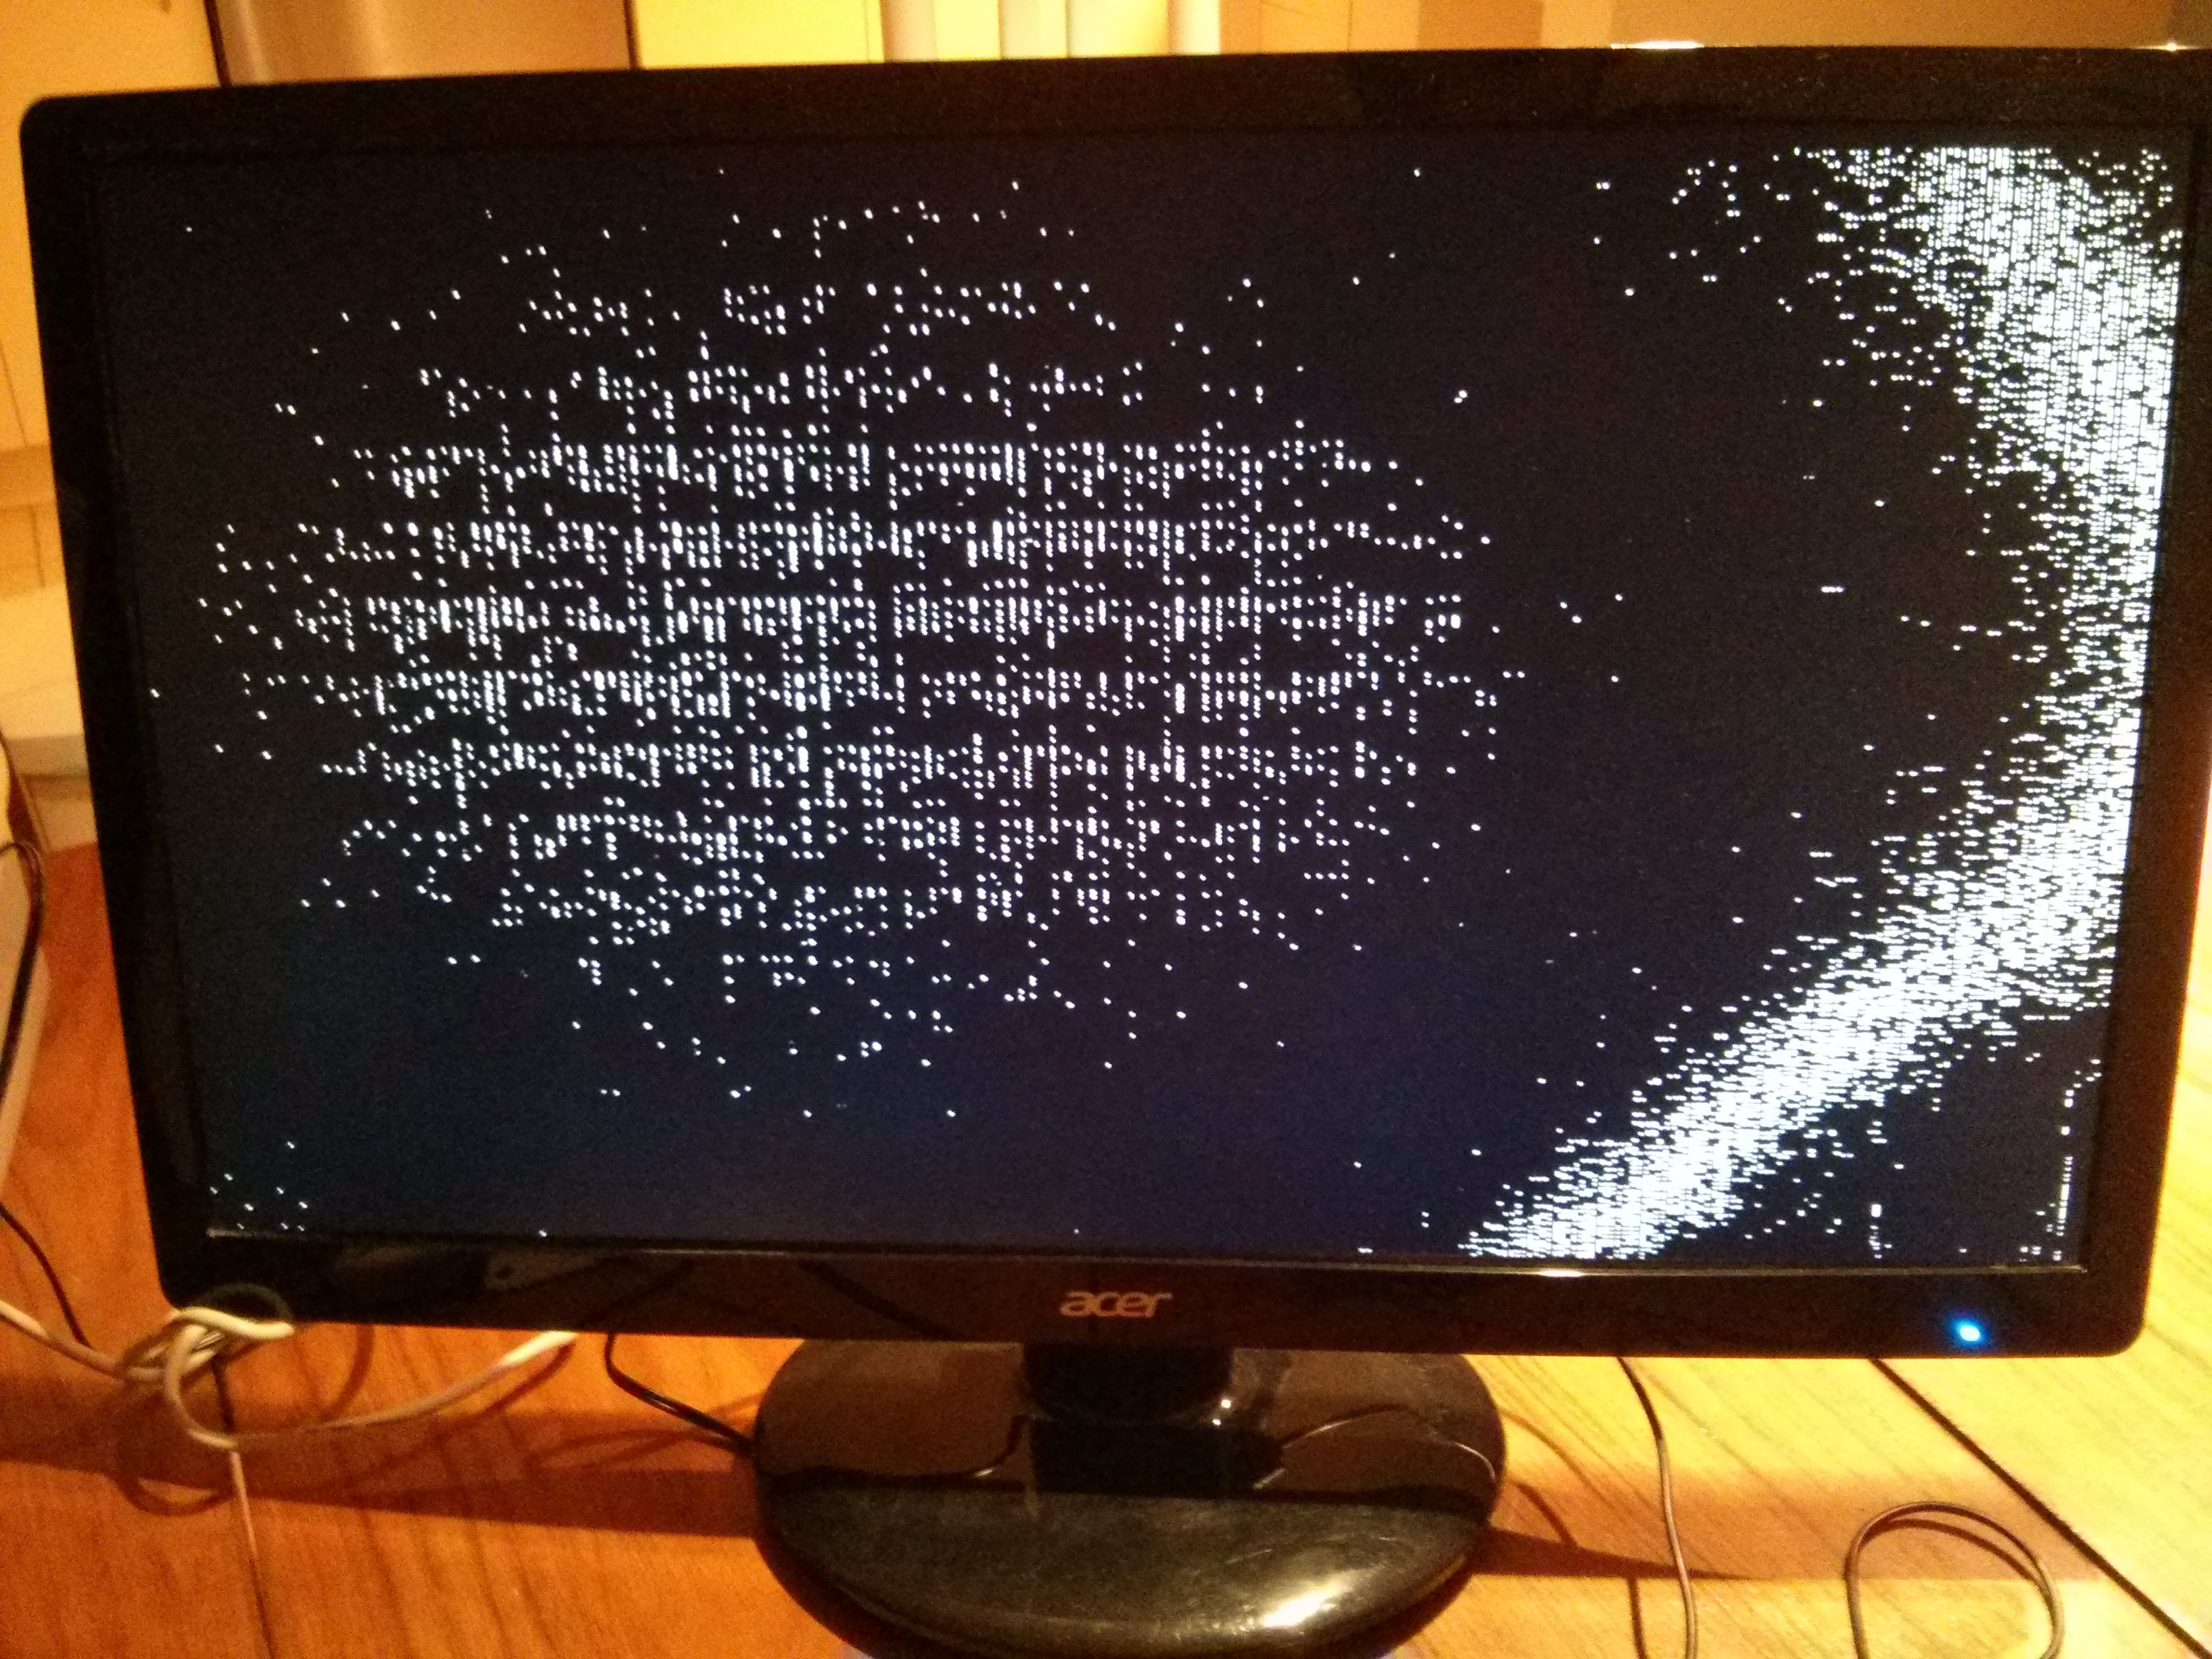
\includegraphics[width=.6\linewidth]{./images/base_no_filter.jpg}
  \caption{Base Frame: No filter}
\end{subfigure}%
\begin{subfigure}{.5\textwidth}
  \centering
  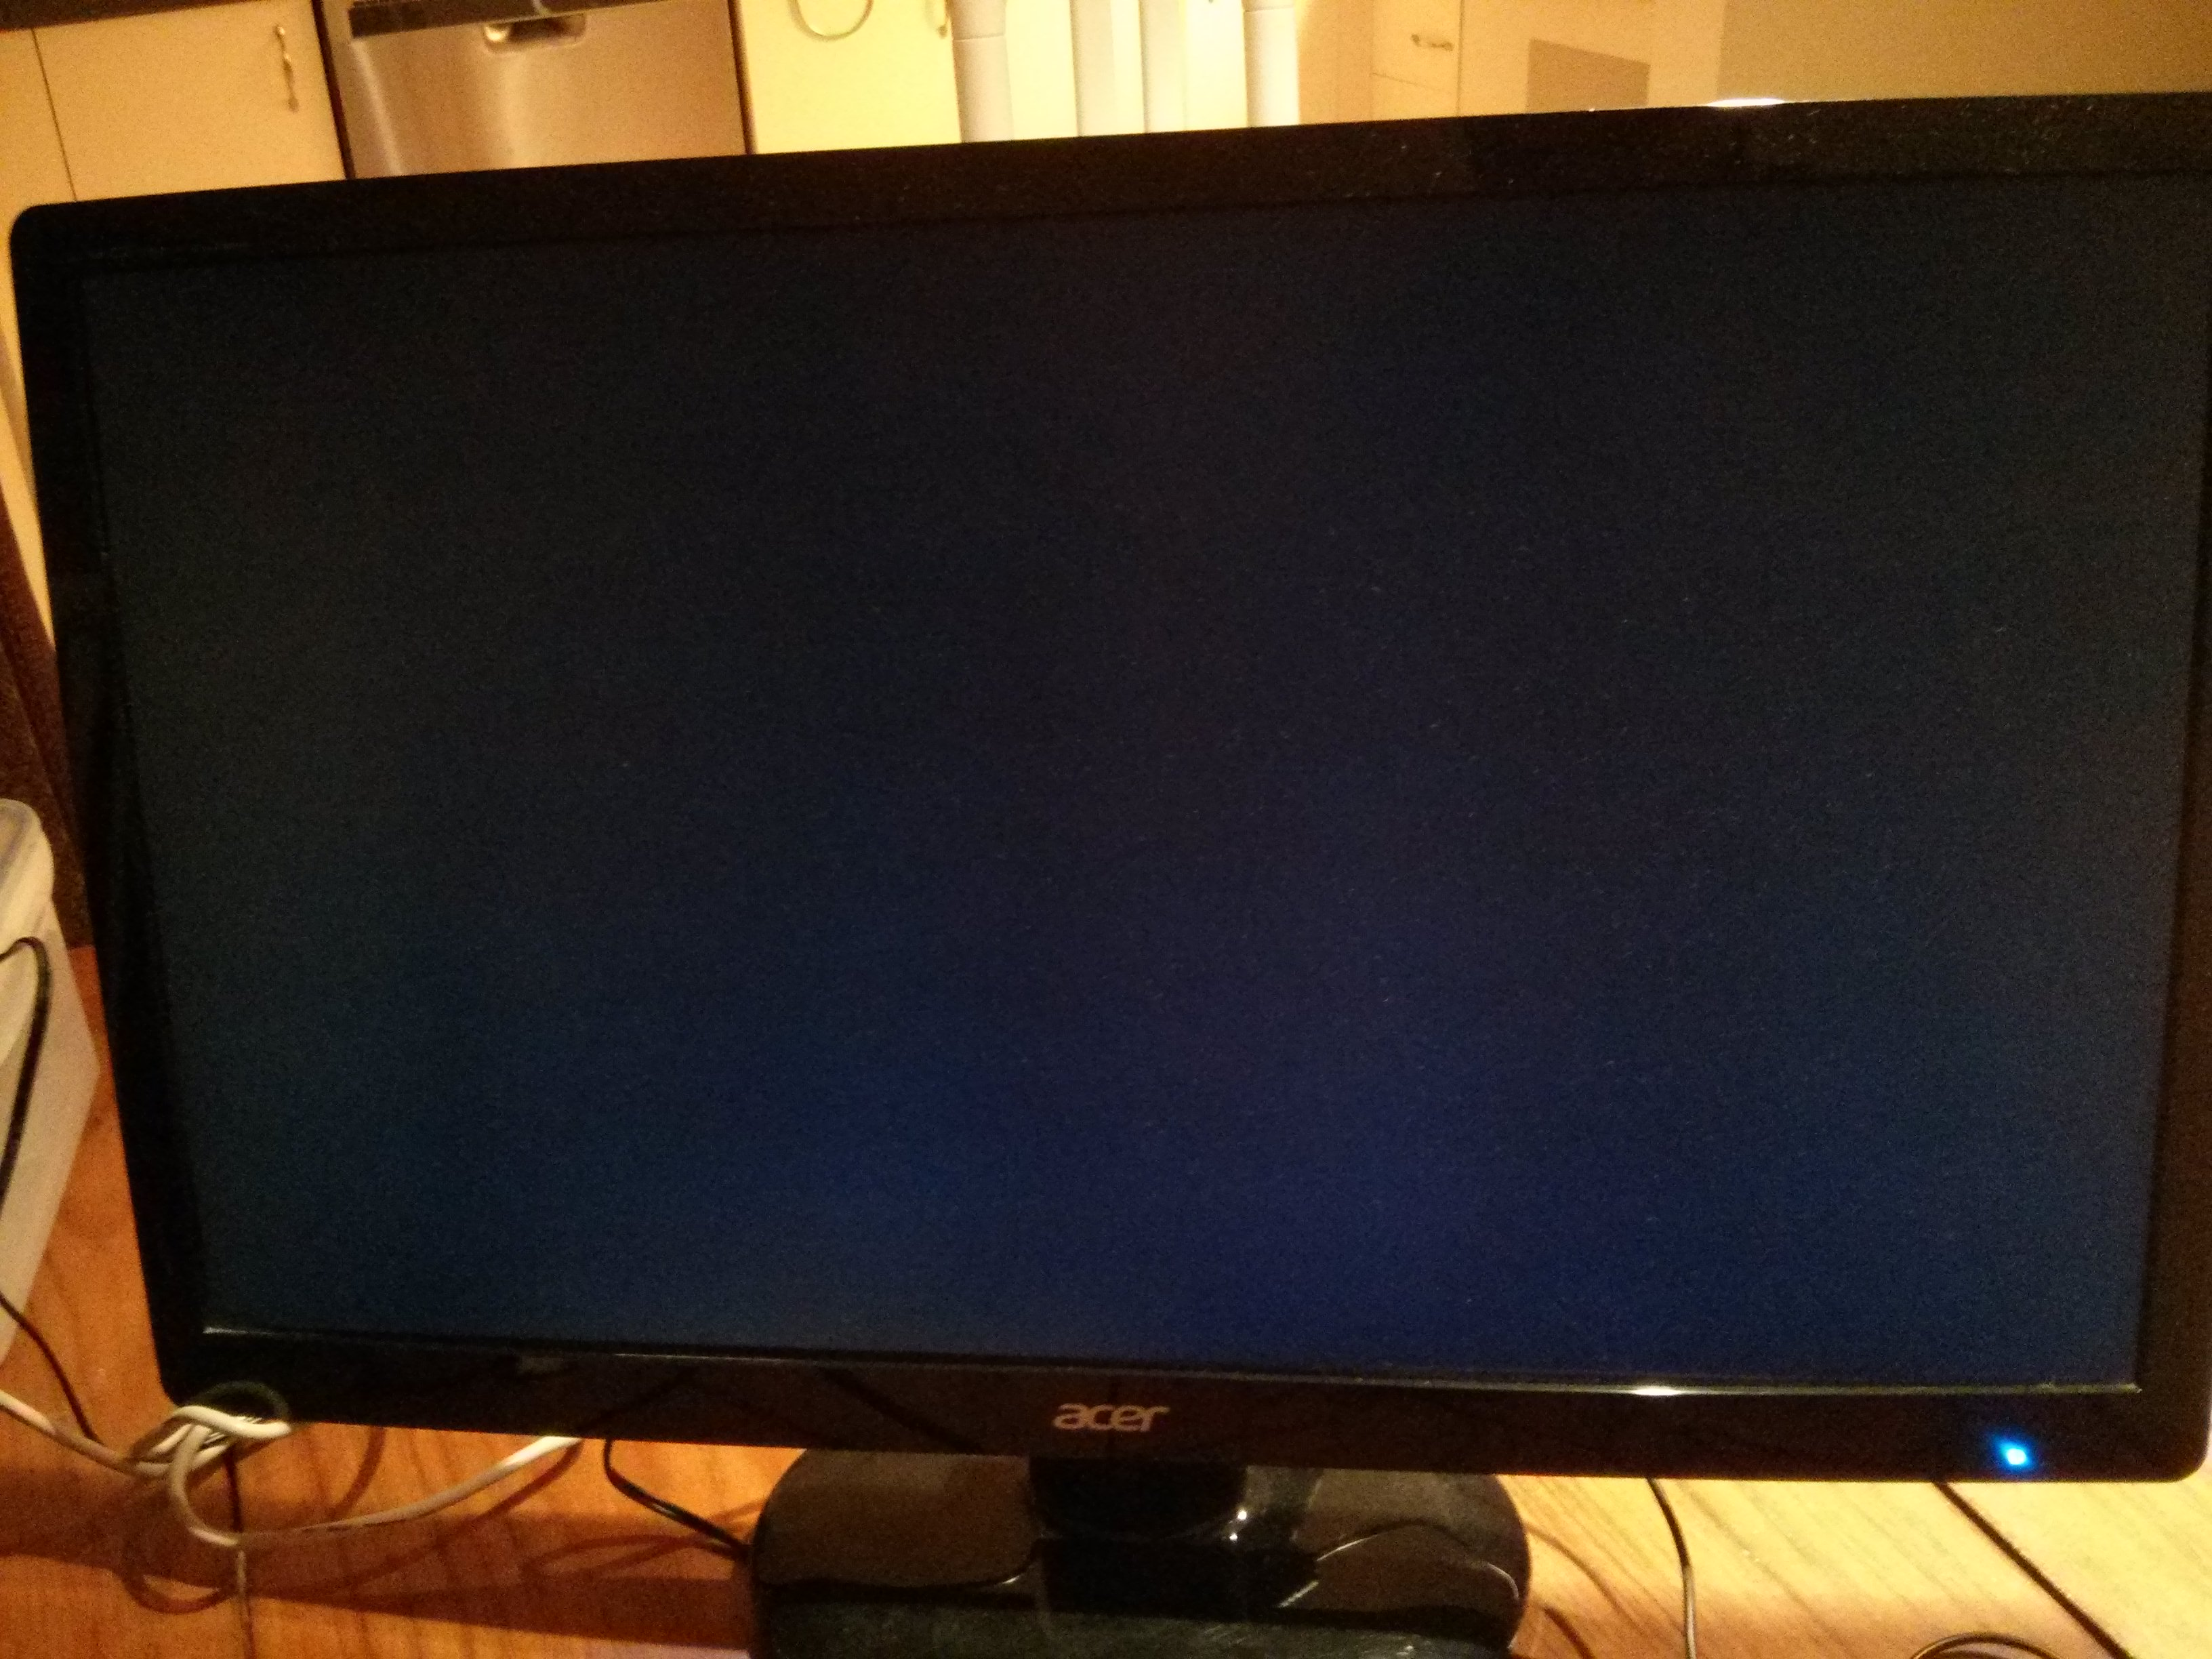
\includegraphics[width=.6\linewidth]{./images/base_filter_20.jpg}
  \caption{Base Frame: Moving average filter of length 20}
\end{subfigure}
\caption{Moving Average Filter}
\label{fig:filter}
\end{figure}
\subsection{Measuring Object Position}
The delta frame data is used to identify the $(x,y)$ coordinates of the object. For this step in the pipeline, one module was designed to calculate the $(x,y)$ coordinate, marking the centre of the object in the frame. Another module was developed to colour the location of the object in the frame for visual identification on the monitor. \\\\
To measure the position of the object, several input data sources were utilized. The input delta frame data is binary. All ones in the delta frame register represent and object pixel, while all zeroes represents the background. When an object pixel is received, the register that holds the total number of object pixels is incremented and the $x$ and $y$ coordinate sum registers are also respectively incremented by the current $x$ and $y$ locations of the object pixel in the frame. The $x$ and $y$ locations are received from the VGA module position outputs. These position sources were used instead of internal counters to ensure that processing is synchronized with the output. Using this process, all the necessary data for equations \ref{eq:x} and \ref{eq:y} are satisfied and the calculation can be preformed under a valid signal condition to obtain the centre of the object. The result is calculated and ready for output when the last pixel in the frame is received and processed. At the beginning of each new frame all data is reset for a fresh calculation. The end of the frame is identified when the $x$ and $y$ location values have reached their max resolution values of 640 and 480 respectively. If no object is in the frame, we don't want to identify noise as an object. To prevent this from happening, a simple threshold was implemented. If the total count of object pixels is less than 40 then the $x$ and $y$ location will be set to a value that is not to be displayed on the monitor. \\\\
The second module utilizes the raw $(x,y)$ coordinates and the updated Kalman $(x,y)$ coordinates to display visual identification of the object on the monitor. The pixels around the raw coordinates are coloured as a red box while the pixels around the Kalman coordinates are coloured as a green box. The incoming $(x,y)$ VGA position coordinate is monitored. If a $(x,y)$ position is within 20 pixels of the object's position, then that pixel is coloured red. The same process is repeated comparing VGA position to Kalman $(x,y)$ coordinates, but instead colouring the pixels green. The result on the monitor shows a red box tracking the object and a green box following the object moving according to the Kalman filter specifications. 
\subsection{Kalman Filter}
The final module developed for the system was the Kalman filter, in the file \texttt{kalman.v}. An in-depth discussion about Kalman filters for object tracking can be found in the Phase 1 report \cite{phase1}, however a brief summary will be provided here. The Kalman filter takes the $(x,y)$ position of the object as input, and computes an improved $(x',y')$ position by using a theoretical model of the system and a characterization of the system error. This is accomplished by iterating through the following set of equations for each input sample. \\\\	
\textbf{Prediction Equations:}
\begin{equation}
\vec{x_{k+1}} = F \cdot \vec{x_k} + B \cdot \vec{u_k}
\label{eq:firstkalman}
\end{equation}
\begin{equation}
P_{k+1} = F \cdot P_k \cdot F^T + Q
\end{equation}
\textbf{Intermediate Calculations:}
\begin{equation}
\vec{y_{k+1}} = \vec{z_k} - H \cdot \vec{x_{k+1}}
\end{equation}
\begin{equation}
S_{k+1} = H \cdot P_{k+1} \cdot H^T + R
\end{equation}
\begin{equation}
K_{k+1} = P_{k+1} \cdot H^T \cdot S_{k+1}^{-1}
\end{equation}
\textbf{Update Equations:}
\begin{equation}
\hat{\vec{x_{k+1}}} = \vec{x_{k+1}} + K_{k+1} \cdot \vec{y_{k+1}}
\end{equation}
\begin{equation}
\hat{P_{k+1}} = (I - K_{k+1} \cdot H) \cdot P_{k+1}
\end{equation}
The model chosen during Phase 1 of the project is constant velocity (i.e. the assumption is made that the object with travel with constant velocity). This means that the state vector, $\vec{x}$, has 4 states: position and velocity in both x and y directions. This means that matrices like $P$ and $F$ are $4 \times 4$, and the matrix math requires many computations. This represents one of the main challenges for hardware implementation of the Kalman filter equations, the shear number of calculations that must take place. This is addressed by "unraveling" the matrix operations using the Verilog \texttt{generate} keyword and lots of loops. The next challenge for hardware implementation of the Kalman filter is that the equations just listed must be completed in a specific, sequential order. To achieve sequential operation using an HDL, a finite-state machine (FSM) must be used. Figure \ref{fig:kalmanFSM} demonstrates the operation of the FSM implemented in \texttt{kalman.v}.
\begin{figure}[h]
\centering
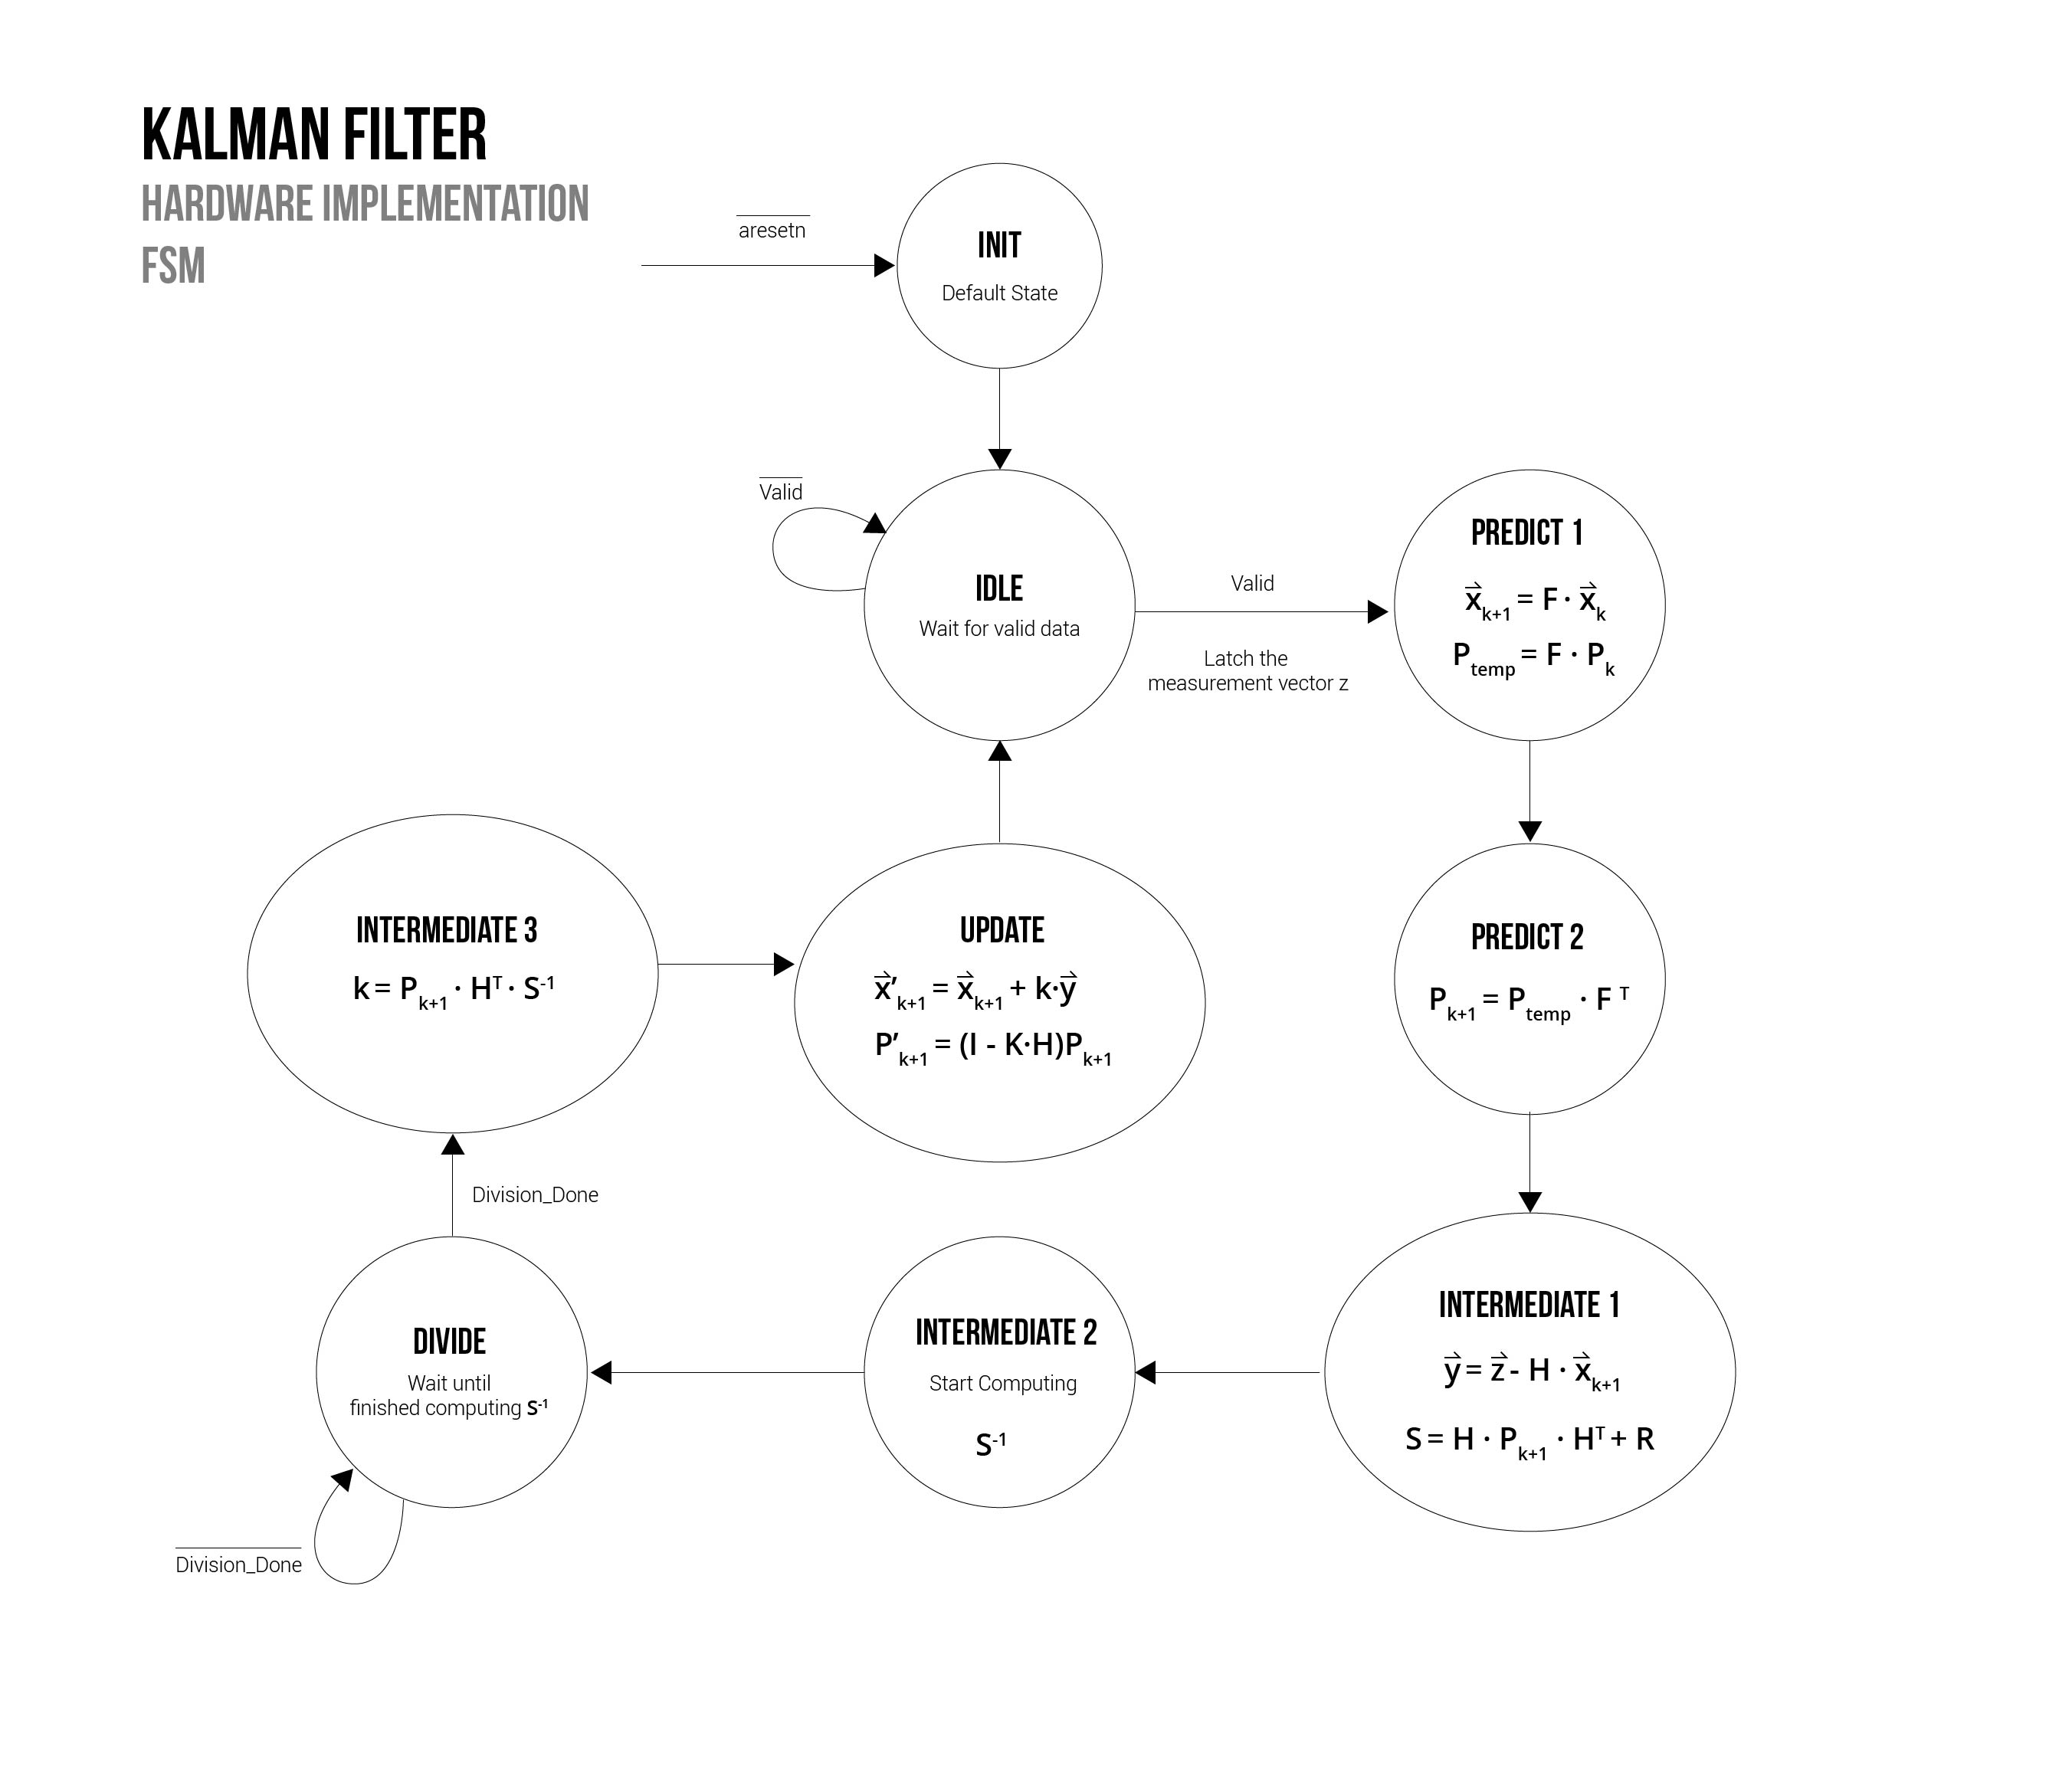
\includegraphics[width=0.8\textwidth]{./images/kalman_fsm.jpg}
\caption{Kalman Filter Finite-State Machine}
\label{fig:kalmanFSM}
\end{figure}
The final, and perhaps most difficult, challenge in designing this module is using fixed-point math. Floating point math requires lots of FPGA resources due to large word length of operands and complex hardware for operations. Fixed-point architecture is characterized by the number of bits used to represent the integer portion, and the number of bits used to represent the fractional portion. Typically this is stylized as $(W, F)$, where the binary string contains $W$ bits, $W-F$ integer bits, and $F$ fractional bits. The need for fixed-point math is introduced in two key places of the Kalman filter equations. The first is the theoretical model matrix, $F$. In this matrix, a value must be used to represent the time step between measurements. Since one measurement occurs per frame and the frame rate is 60 Hz, this time step is 16.6 ms. Since the value is less than one, a fractional portion is needed. Similarly, the Kalman filter equations require computing a matrix inverse, $S^{-1}$. Since $S$ is a $2 \times 2$ matrix, the inverse can be calculated with the formula,
\begin{equation}
S^{-1} = \frac{1}{ad - bc}
\begin{bmatrix}
d & -b \\
-c & a \\
\end{bmatrix}.
\label{eq:inv}
\end{equation}
Again, a value that is less than one will occur, and a fractional portion is needed. Fortunately, the challenge of fixed-point arithmetic was addressed by using a fixed-point Verilog library developed by Tom Burke and Sam Skalicky on \href{http://opencores.org/websvn,filedetails?repname=verilog_fixed_point_math_library&path=%2Fverilog_fixed_point_math_library%2Ftrunk%2FReadMe.txt}{OpenCores}. Specifically, the library modules for fixed-point addition, multiplication, and division were implemented in the Kalman filter for all of the equations. The library assumes data is represented in the $(W,F)$ architecture with the top most bit used for sign. Both input operands must have the same architecture, and the result is returned with the same architecture. The addition (which also can perform subtraction by flipping a sign bit) and multiplication modules are strictly combinational and add no overhead. However, the division module does require $W+F+1$ clock cycles to compute the result, and has control signals to start and finish the operation. \\\\
The Kalman filter module was validated using functional simulation. A testbench was written to put a repeating $(x,y)$ coordinate into the module and the result was observed. The software implementation of the Kalman filter equations, developed in Phase 1, was also tested with the same number of iterations and the same $(x,y)$ pair. The system was validated by comparing the hardware simulation against the software results. The specifics of the simulation will be discussed in section \ref{sec:sim}. \\\\ 
The first working attempt had a fixed-point architecture of $(37, 15)$. This is due to the fact that the maximum value occurring in this first attempt was on the order of 4 million. This value is introduced when computing the determinant of the $S$ matrix. The $S$ matrix has the following form:
\begin{equation}
S = 
\begin{bmatrix}
X & 0 \\
0 & X \\
\end{bmatrix}
\end{equation}
Where $X$ is on the order of 2000. So when computing the determinant in equation \ref{eq:inv}, this maximum value is reached. In order to properly represent this number, 21-bits of integer portion are needed. On the first attempt the fractional portion was arbitrarily set and not optimized. This architecture was clearly too large, and needed to be optimized. Optimization could be performed due to the consistent form of the $S$ matrix just described. Computing the inverse of $S$ always gave a matrix with the same form:
\begin{equation}
S^{-1} = 
\begin{bmatrix}
\frac{1}{X} & 0 \\
0 & \frac{1}{X}  \\
\end{bmatrix}
\end{equation}
Since this form always holds, it was realized that there is no need to compute the determinant of $S$ (i.e. no need to square $X$). This allowed the max integer portion to be reduced to 11-bits, which is much more logical since it is the number of bits needed to represent any location on the display. The minimum value can also be derived from this $S$ matrix. It was found that the fractional portion could be reduced to 12-bits without any problems. This number of bits also stems from the $S$ matrix, since roughly 11-bits are needed to represent $\frac{1}{2000}$, with some room for fluctuations. Thus, the final fixed-point architecture of the Kalman filter is $(24, 12)$. The completed system design can be seen in appendix \ref{sec:finalPipe}. This figure shows the video pipeline after Kalman filter integration. The orange boxes represent Terasic modules, the red boxes represent off FPGA hardware, and the blue boxes represent modules developed during this project. Integrating the Kalman filter caused no issues after it was validated in simulation.
\section{Testing \& Verification}
\label{sec:sim}
As discussed throughout section \ref{sec:design}, the system was validated through a combination of functional simulation and qualitative analysis (i.e. trial and error). Specifically, table \ref{table:testing} shows how each of the experiments discussed in section \ref{sec:design} were validated. While ideally the design flow would always include simulation prior to system integration, in many cases this was not possible since the system requires an analog input signal for stimulation, which we did not have a model for. Thus, any experiment involving the video pipeline had to be validated qualitatively. \\\\
\begin{table}[h]
\centering
\caption{System Validation Summary}
\label{table:testing}
 \begin{tabular}{ | p{6cm} | p{4cm} |} \hline
 \textbf{Experiment} & \textbf{Validation Method}  \\ \hline
VGA Display & Qualitative \\ \hline
Basic Video Input/Output & Qualitative \\ \hline
Modified Pipeline \#1 & Qualitative \\ \hline
RGB to Grayscale Conversion & Simulation \\ \hline
SRAM Controller & Simulation \\ \hline
Modified Pipeline \#2 & Qualitative \\ \hline
Object Measurement & Qualitative \\ \hline
Kalman Filter & Simulation \\ \hline
\end{tabular}
\end{table}
The Kalman filter will be used to show an example of the simulation validation process. The first step is to write a testbench which will stimulate the module under test. For this project, testbenches were written in SystemVerilog, as the language allows use of higher-level abstractions like mailboxes. Next, a DO file is written to list the signals that need to be displayed on the waveform window. The Verilog source is compiled, and Modelsim is used to visualize the input, output, and internal signals of interest. The waveforms are then compared to the result of a software test that matches the functionality of the SystemVerilog testbench. For the Kalman filter module, with the state vector initialized to $[10,10,10,10]$, 10 iterations with the same input value of $(370,350)$ produces the following waveform in figure \ref{fig:wave}.
\begin{figure}[h]
\centering
\caption{Kalman Filter Simulation: 10 Iterations of $(370,350)$}
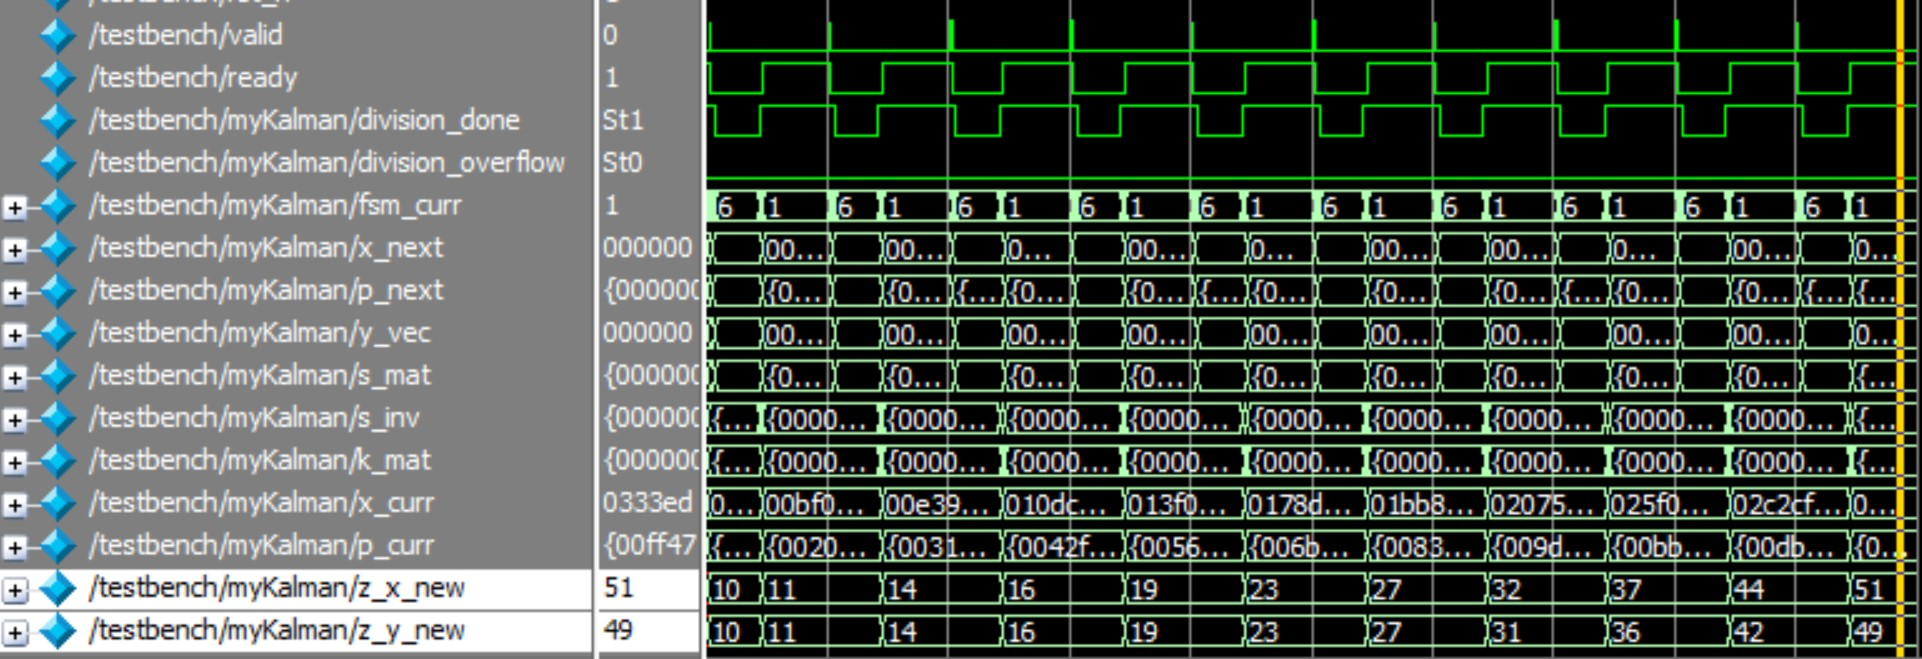
\includegraphics[width=0.8\textwidth]{./images/kalman_sim.jpg}
\label{fig:wave}
\end{figure}
The corresponding software test and result is shown in appendix \ref{sec:software}. Since this result roughly matches the waveform in figure \ref{fig:wave}, the Kalman filter module is functioning correctly. The results are not the exact same due to the fact that the MATLAB code in this case is floating point, double precision. Due to flaws in our fixed-point software developed in Phase 1, we were not able to use it as a bit accurate model. This is an example of the process taken throughout the project for hardware validation using simulation, and it was successful where applicable.
\section{Impact on Society}
Since the scope and application of the project did not change between Phases 1 and 2, discussion of the project's impact on society is entirely based off of the Phase 1 report \cite{phase1}. \\\\
Our dedicated hardware object tracking system will have some impacts in society, but no profound negative impacts. The most notable impact will be its automating effect in the applications it is integrated with. Its introduction to another system will fulfill a task that could have been previously accomplished by a human or even by software previously embedded within the system. The consumer would have to purchase our hardware to implement our system. Our choice of hardware, the Altera DE2 Board has an upfront cost of around \textdollar500. This can be a substantial price for the consumer but the performance benefits outweigh that of embedded software, and in the case of surveillance for example, the cost of running our system will be less than paying a worker to watch a video feed for objects. The introduction of new technology that makes a manned job obsolete is often viewed as a negative impact on society, but this sort of progress is inevitable. \\\\
In the design process so far, we have not made any sort of environmental impact as we have just been developing software. Our system is going to be a combination of previously manufactured parts which were presumably made with the environment in mind. There are so many electronics already in use in society today, the addition of our system's environmental impact can not be quantified. Our product does not produce waste nor does it need constant physical additions. It requires a small constant supply of electricity. When it is no longer needed it can be properly recycled in the same way that computers and other electronics are. Our system does not pose any health or safety risks.\\\\
As mentioned earlier, the value of our device comes from the additional performance gained by a secondary system using it. It is possible that the secondary system has some sort of malicious intent but our product cannot be responsible for any negative consequences the secondary system produces. 
\section{Allocation of Work}
The majority of the hardware implementation this semester was done by Ben with Taylor providing some assistance. Ben was more skilled with hardware description languages and was able to setup the monitor-FPGA interface early on. This required a lot of work and was necessary before we could begin with algorithm implementation. Once the setup was done, the modules were divided between us and were worked on and tested separately. Some modules required both of us to collaborate. Taylor developed the RGB to grayscale module and the measure position module. Ben developed the SDRAM controller, delta frame generation and filtering module, colour position module, and VGA sync module as well as incorporating the sample Terasic modules. The Kalman filter module was worked on by both of us but with Ben spending more individual time on the finite state machine for it. The fixed point library implementation and logic was handled by Ben for the whole pipeline. Both of us participated in several work sessions were we would brainstorm ideas, debug, and test the system. Collaboration and version control was done through a Github repository. For documentation, the progress reports were split evenly. The poster was designed by Taylor with Ben contributing content. For the final report Taylor was assigned a few sections with the majority being written by Ben. No significant teamwork issues were encountered as we were able to meet all deadlines and accomplish our goals.
\section{Conclusion}
The final hardware implementation was a success, and the system can display a red dot that shows the $(x,y)$ measurement of the object in the frame as well as green dot showing the improved $(x',y')$ position the Kalman filter produces. The FPGA resource utilization of the final system is 18\% of available logic, 36\% of available pins, and less than 1\% of the distributed RAM. Due to the underlying principles of the delta frame generation, the system is an object tracking algorithm and not a motion tracking algorithm. However, the Kalman filter theoretical model assumes constant velocity.This is why when the object stops moving, the green dot slowly converges to the red one. This shows the system favoring the measurements over the model to reduce error, and demonstrates the Kalman filter functioning properly. When the object is moving with constant velocity, the Kalman filter provides a smoother, improved output. Appendix \ref{sec:links} has links to videos demonstrating the final hardware system as well as a link to the project repository, which contains all project source files.
\subsection{Future Work}
\subsubsection{Underlying Algorithm}
The system could be significantly improved by using an object measurement algorithm that has fewer requirements and assumptions regarding the environment. To produce a valid delta frame, the scene background must have constant lighting and no objects in it. In a real-time situation, we found it very difficult to ensure these requirements were met. 
\subsubsection{Motion Tracking}
The delta frame generation algorithm detects objects in the scene regardless of whether or not they are in motion. However the Kalman filter assume a constant velocity model, which means that when it receives measurements they might break this model. In order to ensure the scene reflects the model, the underlying algorithm just mentioned could be modified to be a motion tracking algorithm instead of an object tracking algorithm. We have discussed and attempted to implement this by simply constantly grabbing a new base frame. The idea is that if the base frame is updated very frequently, only objects in motion will be measured.
\subsubsection{Feature or Color Detection}
Using specific color or feature detection could be a major system improvement, and would be more useful for applications like surveillance. The simple averaging algorithm implemented for object measurement assumes highly symmetric objects and is perhaps the simplest possible way of locating an object in a scene. This improvement would require more complicated video processing, and using color would require major changes to the system architecture, which was designed for grayscale.
\newpage
\begin{thebibliography}{11}
\bibitem{1}
F. Roth, “Using low cost FPGAs for realtime video processing”, M.S. thesis, Faculty of Informatics, Masaryk University, 2011.
\bibitem{2}
A. Saeed et al., “FPGA based Real-time Target Tracking on a Mobile Platform,” in 2010 International Conference on Computational Intelligence and Communication Networks, 2010, pp. 560-564.
\bibitem{3}
”Video and Image Processing Design Using FPGAs.” Altera. 2007. January 2014. 
http://www.altera.com/literature/wp/wp-video0306.pdf  
\bibitem{4}
E. Trucco and A. Verri, “Chapter 8 - Motion,” in Introductory Techniques for 3D Computer, pp. 177- 219.
\bibitem{5}
S.A. El-Azim et al., “An Efficient Object Tracking Technique Using Block-Matching Algorithm”, in Nineteenth National Radio Science Conference, Alexandria, 2002, pp. 427 - 433.
\bibitem{6} 
Caner et al., “An Adaptive Filtering Framework For Image Registration”, IEEE Trans. Acoustics, Speech, and Signal Processing, vol. 2, no. 2, 885-888. March, 2005. 
\bibitem{7}
Yin et al. \textit{Performance Evaluation of Object Tracking Algorithm} [Online]. Available: http://dircweb.kingston.ac.uk/ 
\bibitem{8}
G. Shrikanth, K. Subramanian, “Implementation of FPGA-Based object tracking algorithm,” Electronics and Communication Engineering Sri Venkateswara College of Engineering, 2008.
\bibitem{9}
E. Pizzini, D. Thomas, “FPGA Based Kalman Filter,” Worcester Polytechnic Institute, 2012.
\bibitem{10}
M. Shabany. (2011, December 27). \textit{Floating-point to Fixed-point Conversion} [Online]. Available: http://ee.sharif.edu/~digitalvlsi/Docs/Fixed-Point.pdf
\bibitem{11} 
N. Devillard. (1998, July). \textit{Fast median search: an ANSI C implementation} [Online]. Available: http://ndevilla.free.fr/median/median.pdf
\bibitem{12}
D. Kohanbash. (2014, January 30). \textit{Kalman Filtering - A Practical Implementation Guide (with code!)} [Online]. Available: http://robotsforroboticists.com/kalman-filtering/
\bibitem{itu} Recommendation ITU-R BT.656-5 (12/2007). “Interface for digital component video signals in 525-line and 625-line television systems operating at the 4:2:2 level of Recommendation ITU-R BT.601". 
\bibitem{sram} ISSI Datasheet: “1M x 16 High-Speed Asynchronous CMOS Static RAM with 3.3V Supply".
\bibitem{vga} \textit{VESA and Industry Standards and Guidelines for Computer Display Monitor Timing (DMT)}, Video Electronics Standards Association, Version 1, Revision 11.
\bibitem{phase1} B. Brown \& T. Dotsikas, “A Real-Time Object Tracking System”, ECSE 456 Final Report, unpublished.
\end{thebibliography}
\newpage
\appendix
\appendixpage
\section{Final Video Pipeline}
\label{sec:finalPipe}
\begin{figure}[h]
\centering
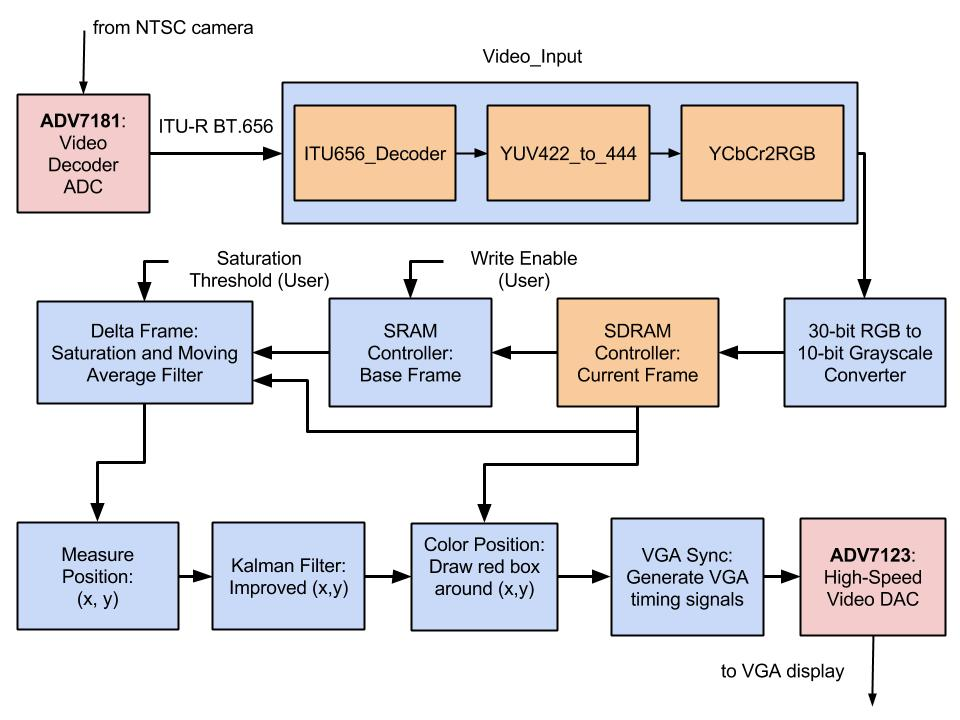
\includegraphics[width=0.8\textwidth]{./images/final_pipeline.jpg}
\end{figure}
\section{Project Resources}
\label{sec:links}
\href{https://github.com/bbrown1867/ObjectTracking}{Project Repository} \\\\
\href{https://www.youtube.com/watch?v=8xPpoj7ziko}{Video: Hardware Implementation - Pre-Kalman Filter} \\\\
\href{https://www.youtube.com/watch?v=48JgtHcgVmo}{Video: Hardware Implementation - Post-Kalman Filter} \\\\
\vspace{3 cm}
\section{Kalman Filter Software Validation}
\label{sec:software}
\subsection{Test Code}
\begin{lstlisting}
x_old = [10; 10; 10; 10];
P_old = eye(4);
t_step = 1 / 64.4;

for i = 1 : 10

    z = [370; 350];

    [x_new, P_new] = applyKalman(z, x_old, P_old, t_step);

    x_old = x_new;
    P_old = P_new;

    str = sprintf('Iteration #%d: (x,y) = (%d, %d)', i, floor(x_new(1)), floor(x_new(2)));
    disp(str);
end
\end{lstlisting}
\subsection{Test Code Trace}
\begin{verbatim}
>> test
Iteration #1: (x,y) = (10, 10)
Iteration #2: (x,y) = (12, 12)
Iteration #3: (x,y) = (13, 13)
Iteration #4: (x,y) = (15, 15)
Iteration #5: (x,y) = (17, 17)
Iteration #6: (x,y) = (20, 19)
Iteration #7: (x,y) = (23, 22)
Iteration #8: (x,y) = (26, 25)
Iteration #9: (x,y) = (30, 28)
Iteration #10: (x,y) = (33, 32)
\end{verbatim}
\end{document}
